% !TEX TS-program = pdflatex

\documentclass[11pt]{amsart}
\usepackage{hyperref}
\usepackage[letterpaper,left=1in,right=1in,top=1in]{geometry}

\usepackage{tikz}
\usetikzlibrary{positioning,chains,fit,shapes,calc,arrows,patterns}
\usepackage{tkz-graph}
\usetikzlibrary{arrows, petri, topaths}
\usepackage{tkz-berge}
\usepackage{tabularx}
\usepackage[all]{xy}
\usepackage{amssymb}


\begin{document}

\begin{center}
\bf Current Problem Sets
\end{center}
\vskip 10 pt

General instructions: Write up the solutions for the problems in each lesson. Scan the work
into a pdf file.  No other file format is accepted. If there are multiple pages for an assignment, merge the pages into a single pdf. 
Upload your work to Blackboard.  Give the file an identifying name such as MyNameMath208L01.pdf
(the L01 is for Lesson 1).
Be sure to save the file with such a name on your computer, not just in Blackboard, since the name of the file
on  your computer will be the name it will have when it is downloaded from Blackboard.  

Make sure the work is dark enough to be read. Use a dark pen or pencil, or
maybe increase the contrast on the scanner.  Show the work that leads to the solution; correct answers without necessary work will earn little if any credit.

 Remember that you cannot expect more than three assignments
to be graded in any seven day period. Graded assignments will be available through Blackboard.

Problems 1 through 5 are worth are worth $5$ points each. Problem 6 is a bonus problem worth $3$ points. The total score for a problem set cannot be greater than $25$.

Sample exercises with solutions are found in an appendix to the text. When solving the problems in this list,
you may use any facts given in the text {\bfseries exercises} \underbar{but not in the text {\bfseries problems}}.
If you want to use a fact in a problem, give a solution to the problem as part of your work. 

\medskip
\begin{center} 
Problems to be submitted.
\end{center}
\medskip



\section{Lesson 1}

\begin{enumerate}


\item Determine which of the following sentences are propositions. Give a brief reason for your answer.
\begin{enumerate} 

\item Seven is two more than five.\\
{\color{blue} This is a proposition. In fact, it is true.}\\

\item Stop whining!\\
{\color{blue} This is not a proposition. It is a command.}\\

\item There is a black hole at the center of every galaxy.\\
{\color{blue} This is a proposition. Its truth value is not currently known.}\\

\item This sentence has five words. \\[10pt]
{\color{blue} This is a proposition. It refers to itself, but in this\\
case there is no question about its truth value: it is true.}\\

\end{enumerate}


\item Construct truth tables for each of the following.

\begin{enumerate} 

\item $\neg q\longrightarrow p$.\\[3pt]

{\color{blue}
\begin{tabular}{@{ }c@{ }@{ }c  | c@{ }@{ }c@{ }@{ }c@{ }@{ }c@{ }@{ }c@{ }@{ }@{ }c}
p & q &  & $\lnot$ & q & $\rightarrow$ & p & \\
\hline
T & T &  &  F & T & \textcolor{red}{T} &  T & \\
T & F &  & T & F & \textcolor{red}{T} &  T & \\
F & T &  & F &  T & \textcolor{red}{T} &  F & \\
F & F &  &  T & F & \textcolor{red}{F} &  F & \\
\end{tabular}\\[5pt]
}


\item $(p\lor q)\longrightarrow  r$. 
(You will need eight rows for this one.)\\[10pt]
{\color{blue}
\begin{tabular}{@{ }c@{ }@{ }c@{ }@{ }c | c@{ }@{}c@{}@{ }c@{ }@{ }c@{ }@{ }c@{ }@{}c@{}@{ }c@{ }@{ }c@{ }@{ }c c@{}@{ }cc@{}@{ }c@{ }c}
p & q & r &  & ( & p & $\lor$ & q & ) & $\to$ & r  & \\
\hline
T & T & T &  &  & T & T & T &  & \textcolor{red}{T} & T  &  & \\
T & T & F &  &  & T & T & T &  & \textcolor{red}{F} & F &  &   \\
T & F & T &  &  & T & T & F &  & \textcolor{red}{T} & T &  &   \\
T & F & F &  &  & T & T & F &  & \textcolor{red}{F} & F &  &  \\
F & T & T &  &  & F & T & T &  & \textcolor{red}{T} & T &  &   \\
F & T & F &  &  & F & T & T &  & \textcolor{red}{F} & F &  &   \\
F & F & T &  &  & F & F & F &  & \textcolor{red}{T} & T &  &   \\
F & F & F &  &  & F & F & F &  & \textcolor{red}{T} & T &  &   \\
\end{tabular}\\[5pt]
}

\end{enumerate}


\item Let $s$ be the proposition {\itshape It is snowing}, $f$ be the proposition 
{\itshape It is below freezing}, and $r$ be {\itshape It is raining}. Convert the following English sentences into statements
using the symbols $s$, $f$, $r$ and logical connectives.

\begin{enumerate}

\item It is snowing or it is not below freezing.\\
{\color{blue} $s \lor \lnot f$}\\

\item If it is snowing, then it is not raining and it is below freezing.\\
{\color{blue} This one is ambiguous. 
Either $s \to (\lnot r \land f)$ or $(s \to \lnot r) \land f$ would be ok.
But\\
 parentheses are needed in either case, and the first one is the 
{\itshape natural} choice.}\\[7pt]

\end{enumerate}

\item  Use a truth table to verify  the  equivalence:
$p\longrightarrow \neg q\equiv \neg p\lor\neg q$.\\
Explain why the truth table shows that the propositions are equivalent.\\[10pt]
{\color{blue}
$\vbox{\offinterlineskip
\halign { \strut # & # & \vrule ~# & \vrule {\color{red} ~~#} & \vrule ~# & \vrule{\color{red}  ~#} \cr
$p$ & $q$ &  $\lnot q$ & $p \rightarrow \lnot q$ &  $\lnot p$ & $\neg q \lor \neg p$ \cr
\noalign{\hrule}
T   &  T   &  F & F  &  F  & \,F \cr
T   &  F   &  T & T  &  F  & \,T \cr
F   &  T   &  F & T  &  T  & \,T \cr
F   &  F   &  T & T  &  T  & \,T \cr
}}$\\[3pt]

Since the two columns shown in red are identical, we see $p\longrightarrow \lnot q\equiv \lnot p\lor \neg q$.
}\\[5pt]


\item Use a truth table to show that the statements $p\longrightarrow (q\longrightarrow r) \text{ and  }(p\longrightarrow q)\longrightarrow r$ \\
are not logically equivalent. \\
Explain why the truth table shows that the propositions are not equivalent.\\[10pt]
{\color{blue}
$\vbox{\offinterlineskip
\halign { \strut # & # & # & \vrule ~~# & \vrule {\color{red} ~~#} & \vrule ~~# & \vrule {\color{red} ~~#}  \cr
$p$ & $q$ & $r$ & $q\rightarrow r$ & $p\rightarrow (q\rightarrow r)$ & $p\rightarrow q$ & $(p \rightarrow q)\rightarrow r$ \cr
\noalign{\hrule}
T   &  T   &  T   &  T  &  T  & T &  T\cr
T   &  T   &  F   &  F  &  F   & T & F\cr
T   &  F   &  T   &  T  &  T   & F & T\cr
T   &  F   &  F   &  T  &  T   & F & T\cr
F   &  T   &  T   &  T  &  T  & T & T\cr
F   &  T   &  F   &  F  &  T  & T & F\cr
F   &  F   &  T   &  T  &  T  & T & T\cr
F   &  F   &  F   &  T  &  T  & T & F\cr
}}$\\[3pt]
The columns in red are not identical, we see $p\longrightarrow (q\longrightarrow r) \text{ and  }(p\longrightarrow q)\longrightarrow r$ are not logically equivalent. 
}\\[10pt]



\item ({\bf bonus}) Give a proof of the following equivalence following the pattern
of proof shown in the examples in section 2.6 of the text:  $\neg p\longrightarrow(p\longrightarrow q)\equiv {\bf T}$.\\[10pt]
{\color{blue}\underbar{Solution}:
\begin{align*}
\lnot p\rightarrow (p\rightarrow q)
& \equiv \lnot\lnot p \lor  (\lnot p\lor q)         &\text{Disjunctive Form (twice)}\\
&\equiv p \lor (\lnot p\lor q)                           &\text{Double Negation}\\
&\equiv (p\lor \lnot p)\lor q                            &\text{Associative Law}\\
&\equiv {\mathbb T} \lor q                              &\text{Law of Excluded Middle}\\
&\equiv q \lor {\mathbb T}                              &\text{Commutative Law}\\
&\equiv {\mathbb T}                                        &\text{Domination Law}
\end{align*}
}

\end{enumerate}

\section{Lesson 2}

\begin{enumerate}

\item Let $P(x): x^2\leq 4$.  The domain for $x$ is all positive integers ($1,2,3,\ldots$). Determine the truth values of the following propositions. 
\begin{enumerate}
\item $P(5)$\\[3pt]
{\color{blue}
$P(5): 5^2 \leq 4$ is false.
}\\[3pt]
\item$\neg \forall x\, P(x)$\\[3pt]
{\color{blue}
In words: Not every integer has a square that is less than or equal to $4$. That is true.
For example $3^2$ is not less than or equal to $4$.
}\\[5pt] 

\end{enumerate}


\item Let $P(x,y)$ be {\it $x$ has read $y$}, where the domain of discourse for 
$x$ is all students
in this class, and the domain of discourse for $y$ is all books written by Mark Twain. Express the
following propositions in English. 
\begin{enumerate}
\item $\forall x\, P(x,\text{Huckleberry Finn}).$\\[3pt]
{\color{blue}
Every student in this class has read Huckleberry Finn.
}\\[3pt]
\item $\exists x\, \forall y\, P(x,y).$\\[3pt]
{\color{blue}
There is a student in this class who has read every book by Mark Twain.
}\\[3pt]
\item $\forall y\, \exists x\, P(x,y).$\\[3pt]
{\color{blue}
For each book by Mark Twain, there is at least one student in the class who has read that book.
}\\[5pt]
\end{enumerate}

\vfill\break

\item Let $F(x,y)$ be the statement {\it $x$ trusts $y$}, where the domain of discourse
for both $x$ and $y$ is  all people. 
\begin{enumerate}
\item
 Use quantifiers to express each of the following propositions in symbols.
\begin{enumerate}
\item Nobody trusts Ralph.\\[3pt]
{\color{blue} $\lnot\exists{x}\,F(x,Ralph)$}\\[3pt]

\item Everybody trusts Fred.\\[3pt]
{\color{blue} $\forall{x}\,F(x,Fred)$}\\[3pt]

\item Somebody trusts everybody.\\[3pt]
{\color{blue} $\exists{x}\forall{y}\,F(x,y)$}\\[3pt]

\end{enumerate}

\item Now write the negation of those propositions in symbols. The cheap way would be to simply write $\lnot$ in front of each of the answers to part (a). Don't do that. Use the rules discussed in the text so your answer does not have $\lnot$ occurring to the left of any quantifiers.\\[3pt]
\begin{enumerate}

\item {\color{blue} $\exists{x}\,F(x,Ralph)$}\\[3pt]

\item{\color{blue} $\exists{x}\,\lnot F(x,Fred)$}\\[3pt]

\item 
{\color{blue} $\forall{x}\exists{y}\,\lnot F(x,y)$}\\[3pt]

\end{enumerate}


\item Express each of those negations in an English sentence.\\[3pt]
\begin{enumerate}

\item {\color{blue} Somebody trusts Ralph.}\\[3pt]

\item {\color{blue} Somebody does not trust Fred.}\\[3pt]

\item {\color{blue} Each person has somebody they don't trust.}\\[5pt]
\end{enumerate}

\end{enumerate}
\vfill\break
\item  Show that {\it $p\longrightarrow q$ and $\neg p,\quad \therefore \neg q$} is not a valid rule
of inference. It is called the fallacy of denying the hypothesis. To expand a bit on the reading for this lesson, here is how to show a proposed rule of inference is valid using a truth table: Construct a truth table with columns for the hypotheses and a column for the conclusion. Check that in every row where the hypotheses all have truth value {\bf T}, the conclusion also has truth value {\bf T}. In plain English, check that if we agree the hypotheses are all true, then the conclusion is true as well. Notice that in rows where the hypotheses do not all have truth value {\bf T}, the truth value of the conclusion does not matter. Flipping that {\it validity test}  around, an argument is not valid if there is a row in the truth table where the hypotheses are all {\bf T}, but the conclusion is {\bf F}. Such a row shows that it is possible to agree that the hypotheses are all true, and yet still have the conclusion false. That means the argument is not valid.\\[5pt]

{\color{blue}
$\vbox{\offinterlineskip
\halign { \strut # & # & \vrule ~# & \vrule  ~~# & \vrule ~# & \vrule  ~# \cr
$p$ & $q$ &  $p \rightarrow q$ &  $\lnot p$ & $\lnot q$ \cr
\noalign{\hrule}
T   &  T   &   T  &  F  & \,F \cr
T   &  F    & F  &  F  & \,T \cr
F   &  T    & {\color{red}T}  & {\color{red} T}  & \,{\color{red}F} \cr
F   &  F    & T  &  T  & \,T \cr
}}$\\[3pt]
For the entries in the third row, both hypotheses are true, but the conclusion is false. That shows the argument 
is not valid.\\[5pt]
}
\vfill\break
\item Express the following argument symbolically, and then prove, using the style of proof shown in \underbar{table} 4.2 of the text,  that the argument is valid.  {\it If Ralph doesn't have a sore shoulder
or he doesn't feel sick, then he will go bowling and  he will go to the movie. If he goes to the movie, he will buy popcorn.  He didn't buy popcorn. So Ralph has a sore shoulder.}

(Use
$s$ for Ralph has a sore shoulder.
$f$ for Ralph feels sick. 
$b$ for Ralph goes bowling.
$m$ for Ralph goes to the movie.
$p$ for Ralph buys popcorn.

Warning: You will probably want to use the rule of Simplification at some point in your proof. You need to be careful with that rule! In plain English, the rule says that if you know $p$ and $q$ is true, then you can conclude $p$ is true. But watch out: if $p \land q$ is part of a larger proposition, you can not replace $p \land q$ with $p$. For example, consider the proposition {\it If I bet \$1000 on My Pony and My Pony wins the race, then I will be rich.} Obviously it is not valid to say, by Simplification, {\it If I bet \$1000 on My Pony, then I will be rich.} So, be careful using Simplification.\\[5pt]

{\color{blue}
\text{Argument:}\\
$(\lnot s \lor \lnot f)\rightarrow (b \land m)$\\
$m \rightarrow p$\\
$\lnot p$\\
\vrule width 1.2truein height 0pt depth .4pt\\[4pt]
$\therefore \, s$\\[3pt]
\textbf{Proof:}
 \begin{tabular}[t]{r l l}
 (1)& $m\rightarrow p$                   & hypothesis\\
 (2)& $ \lnot p$      & hypothesis\\
 (3)& $\lnot m$                   & Modus Tollens (1) and (2)\\
 (4)& $\lnot m \lor \lnot b$ & Addition (3)\\
 (5)& $\lnot(m\land b)$ & De Morgan's Law (4)\\
 (6)& $(\lnot s \lor \lnot f)\rightarrow (m \land b)$              & hypothesis\\
 (7)& $\lnot(\lnot s \lor \lnot f)$             & Modus Tollens (5) and (6)\\
 (8)& $\lnot\lnot s \land \lnot\lnot f$             & De Morgan's Law (7)\\
 (9)& $\lnot\lnot s$                   & Simplification (8)\\
 (10)& $s$            & Double Negation
 \end{tabular}\\[5pt]
}

\vfill\break

\item (bonus) Prove
\begin{align*}
&\exists{x}(A(x)\land\neg B(x))\\[4pt]
&\forall{x}(A(x) \longrightarrow C(x))\\[4pt]
\noalign{\kern -10pt}
&\vrule width 1.2truein height 0pt depth .4pt\\[4pt] 
&\therefore \exists{x}(C(x)\land \neg B(x))\\[4pt]
\end{align*}
Hint: This is very similar to example 4.2 in the text.\\[5pt]

{\color{blue}
\textbf{Proof:}
\begin{tabular}[t]{l l}
1) $\exists{x}(A(x) \land \lnot B(x))$& hypothesis \\
2) $A(t)\land \lnot B(t) \hbox{ for some } t $& Existential Instantiation (1) \\ 
3) $A(t)$& Simplification (2) \\ 
4) $\forall{x}(A(x) \to C(x))$& hypothesis \\ 
5) $A(t)\to C(t)$& Universal Instantiation (4) \\ 
6) $C(t)$& Modus Ponens (3) and (5) \\ 
7) $\lnot B(t) \land A(t)$& logical equivalence (2) \\ 
8) $\lnot B(t)$& Simplification (7) \\ 
9) $C(t)\land \lnot B(t)$& Conjunction (6) and (8) \\ 
10) $\exists{x}(C(x)\land \lnot B(x))$& Existential Generalization (9)
\end{tabular}
}

\end{enumerate}


\section{Lesson 3}

\begin{enumerate}


\item Write the following sets using the roster form:

\begin{enumerate}
\item $\{x \in \mathbb{Z} | 10\leq x^2< 100\}$ (Careful, that is $\mathbb Z$, not $\mathbb N$!)\\[3pt]
{\color{blue} $\{-9, -8, -7 -6 -5, -4, 4, 5, 6, 7, 8, 9\}$}\\[3pt]
\item  $\{x\in \mathbb{N} | x\leq 4\}$ (Remember that, in this text anyhow, $0\in \mathbb{N}$.)\\[3pt]
{\color{blue} $\{0, 1, 2, 3, 4\}\}$}\\[5pt]
\end{enumerate}

\item Use set-builder notation to give a description of each set.
\begin{enumerate}
\item $\{ 4, 8, 12\}.$\\[3pt]
{\color{blue} $\left\{ x \,|\, \frac{x}{4} \in \mathbb{N} \text{ and } 1\leq \frac{x}{4}\leq 3\right\}$}\\[3pt]
\item $\{-2, 0, 2, 4, 6\}.$\\[3pt]
{\color{blue} $\{ x \,|\, x \text{ is an even integer and } -2\leq x\leq 6\}$}\\[5pt]
\end{enumerate}

\vfill\break

\item  Let $A=\{1,2,3,5,6,7\}$ and $B=\{2,4,6,8,9\}$. Find 
\begin{enumerate}
\item $A\cap B$ \\[3pt]
{\color{blue} $\{ 2, 6\}$}\\[3pt]
\item $A\cup B$\\[3pt]
{\color{blue} $\{ 1, 2, 3, 4, 5, 6, 7, 8, 9\}$}\\[3pt]
\item $A-B$\\[3pt]
{\color{blue} $\{1, 3, 5, 7\}$}\\[3pt]
\item $B-A$\\[3pt]
{\color{blue} $\{ 4, 8, 9\}$}\\[3pt]
\end{enumerate}

\item Draw Venn diagrams for $A\cap (B \cup C)$ and $(A\cap B)\cup(A\cap C)$ to  show that $A\cap (B \cup C) = (A\cap B)\cup(A\cap C)$.\\[3pt]

  \def\firstcircle{(90:0.5cm) circle (0.75cm)}
  \def\secondcircle{(210:0.5cm) circle (0.75cm)}
  \def\thirdcircle{(330:0.55cm) circle (0.75cm)}

\raisebox{-1.0cm}
 {   \begin{tikzpicture}
        \fill[cyan] \firstcircle; 
        \draw \firstcircle node[text=black,above] {$A$};
        \draw \secondcircle node [text=black,below left] {$B$};
        \draw \thirdcircle node [text=black,below right] {$C$};
    \end{tikzpicture}
}
$\cap$
\raisebox{-1.0cm}
{   \begin{tikzpicture}  
      \fill[cyan] \secondcircle;
      \fill[cyan] \thirdcircle;  
      \draw \firstcircle node[text=black,above] {$A$};      
      \draw \secondcircle node [text=black,below left] {$B$};
      \draw \thirdcircle node [text=black,below right] {$C$};
    \end{tikzpicture}
}
$=$
\raisebox{-1.0cm}
 {   \begin{tikzpicture}
     \begin{scope}
    \clip \firstcircle;
   \fill[cyan] \secondcircle;
     \end{scope}    
      \begin{scope}
    \clip \firstcircle;
    \fill[cyan] \thirdcircle;
      \end{scope}
      \draw \firstcircle node[text=black,above] {$A$};
      \draw \secondcircle node [text=black,below left] {$B$};
      \draw \thirdcircle node [text=black,below right] {$C$};
    \end{tikzpicture}
}

\vskip 10pt

\raisebox{-1.0cm}
 {   \begin{tikzpicture}
     \begin{scope}
    \clip \firstcircle;
   \fill[cyan] \secondcircle;
     \end{scope}          
      \draw \firstcircle node[text=black,above] {$A$};
      \draw \secondcircle node [text=black,below left] {$B$};
      \draw \thirdcircle node [text=black,below right] {$C$};
    \end{tikzpicture}
}
 $\cup$   
\raisebox{-1.0cm}
 {   \begin{tikzpicture}
     \begin{scope}
    \clip \firstcircle;
   \fill[cyan] \thirdcircle;
     \end{scope}          
      \draw \firstcircle node[text=black,above] {$A$};
      \draw \secondcircle node [text=black,below left] {$B$};
      \draw \thirdcircle node [text=black,below right] {$C$};
    \end{tikzpicture}
}
$=$
\raisebox{-1.0cm}
 {   \begin{tikzpicture}
     \begin{scope}
    \clip \firstcircle;
   \fill[cyan] \secondcircle;
     \end{scope}    
      \begin{scope}
    \clip \firstcircle;
    \fill[cyan] \thirdcircle;
      \end{scope}
      \draw \firstcircle node[text=black,above] {$A$};
      \draw \secondcircle node [text=black,below left] {$B$};
      \draw \thirdcircle node [text=black,below right] {$C$};
    \end{tikzpicture}
}
\vskip 10pt
{\color{blue}
Since the same regions are shaded in the righthand Venn diagram in each row, we see
$A\cap (B \cup C) = (A\cap B)\cup(A\cap C)$.}\\[5pt]


\item Let $A=\{1,2,3,4\}\times\{1,2,3\}$. List the elements of the set
$B= \{ (s,t)\in A\,|\, s\geq t\,\}$.\\[3pt] 
{\color{blue} $B =\{ (1,1), (2,1), (2,2), (3,1), (3,2), (3,3), (4,1), (4,2), (4,3)\}$}\\[5pt]

\item (bonus) Is the proposition {\it Every element of the empty set has 
three toes} true or false? Explain your answer! Hint: In symbols, the proposition is written:
  $\forall x (x\in \emptyset \longrightarrow x \text{ has three toes})$. Think about the truth value of that implication.\\[3pt]
  {\color{blue} $\forall x (x\in \emptyset \to x $ has three toes)
 is true since  $x\in\emptyset$
 is sure to be false, and  $p\to q$  is true if  $p$ is false.
 }\\[5pt]

\end{enumerate}

\section{Lesson 4}

\begin{enumerate}

\item [] For  these exercises, you will need to know the definitions of even and odd integers. 
 An integer $n$ is {\it even} if $n=2k$ for some integer $k$. An integer $n$ is {\it odd}
if $n=2k+1$ for some integer $k$. There are no integers that are both even and odd!
Examples: $6$ is even since $6 = (2)(3)$, $-8$ is even since $-8 = (2)(-4)$, $0$ is even since $0 = (2)(0)$, $3$ is odd since $3 = 2(1)+1$, and $-9$ is odd since $-9 = (2)(-5)+1$.\\[8pt]


\item Give a direct proof that the sum of  an odd integer and an even integer is odd. 

Hint: Start by letting $m$ be an odd integer and letting $n$ be an even integer. That means $m = 2k+1$ for some integer $k$ and $n = 2j$ for some integer $j$. Notice that if we let the odd and even integers be $2k+1$ and $2k$, the proof will only account for the cases in which $n$ is one less than $m$.
That is why we need to have $m = 2k+1$ and $n=2j$ for integers $k,j$, so that the sum of  any odd and any even will be considered. 
You are interested in $m+ n$, so add them up and see what you get.  Why is the thing you get an odd integer (think about the definition of {\it odd})?\\[5pt]

{\color{blue}
Let $m$ be an odd integer and let $n$ be an even integer. That means $m = 2k+1$ and $n=2j$ for some integers $k$ and $j$. So, $m+n = (2k)+(2j+1)
= 2(k+j) + 1$. Since $k+j$ is an integer, that shows $m+n$ is odd.  $\clubsuit$}\\[5pt]

\item Give an  indirect proof that if $n^3$ is even, then $n$ is even. Hint: Study the solution of a similar statement in the sample solutions for this lesson.\\[5pt]

{\color{blue} Suppose $n$ is not even. Then $n$ is odd, and so $n = 2k+1$ for some integer $k$. So
$n^{3} = (2k+1)^{3} = 8k^{3} + 12k^{2} + 6k + 1 = 2(4k^{3}+6k^{2}+3k) +1$, which shows $n^{3}$ is odd. $\clubsuit$\\[5pt]
}


\item Give a proof by contradiction that if $5n-4$ is odd, then $n$ is odd.

Hint:  This is the problem in this set that gives the most grief.  Study the section
in  the  notes  where  the  mechanics  of  proving  a  statement  of  the  form
If P, then Q by contradiction is discussed.  Be sure you understand why the first line of the proof should be something like {\it Suppose $5n- 4$ is odd {\bfseries and} $n$ is even.}\\[5pt]

{\color{blue} Suppose $5n-4$ is an odd integer and $n$ is an even integer. Say $n = 2k$ for an integer $k$. Then 
$5n-4= 5(2k)-4 = 2(5k-2)$. That shows $5n-4$ is even. So it is not odd. Conclusion $5n-4$ is odd and it is not odd. That is a contradiction.
$\clubsuit$}\\[5pt]

\item  Give an example of a predicate $P(n)$ about positive integers $n$, such that
$P(n)$ is true for every positive integer from 1 to one billion, but which is never-the-less not
true for all positive integers.  (Hints:  (1) There is a really simple choice possible for the predicate
$P(n)$, (2) Make sure you write down a {\bfseries predicate} with variable $n$, and not a {\bf proposition}!)
The purpose of this problem is to convince you that when checking a
{\it for all}
type proposition, it is not good enough to just check the truth for a few sample cases,
or, for that matter, even a few billion sample cases.  A general proof that covers all
possible cases is necessary.\\[5pt]

{\color{blue} (one option) $P(n): n\leq 1,000,000,000$ (domain of $n$ is the set of integers)}\\[5pt] 

\vfill\break

\item Give a counterexample to the proposition {\it Every positive
integer that ends with the digits $13$ is a prime.}\\[5pt]
{\color{blue} $213$ ends with $13$ but $213 = (3)(71)$, so $213$ is not a prime.}\\[5pt]

\item(bonus) 
The {\bfseries maximum} of two numbers, $a$ and $b$, is $a$ provided $a\geq b$. Notation: $\max(a,b) = a$. The {\bfseries minimum}
of $a$ and $b$ is $a$ provided $a\leq b$. Notation: $\min(a,b) = a$.  Examples: $\max(2,3) = 3$, $\max(5,0) = 5$, $\min(2,3) = 2$,
$\min(5,0) = 0$, $\max(4,4) = \min(4,4) = 4$.\\
Give a proof by cases (two cases is the natural choice for this problem)  that for any numbers $s,t$,
\[\min(s,t)+\max(s,t) = s+t.\]\\[5pt]

{\color{blue} Consider the two possible cases: $s\leq t$ and $s\geq t$.\\
\underbar{case 1}: Suppose $s\leq t$. Then $\min(s,t) = s$ and $\max(s,t)=t$. That means
\[\min(s,t)+\max(s,t) = s+t.\]\\[3pt]
\underbar{case 2}: Suppose $s\geq t$. Then $\min(s,t) = t$ and $\max(s,t)=s$. That means
\[\min(s,t)+\max(s,t) = t+s = s+t.\]\\[3pt]
So, in any case, $\min(s,t)+\max(s,t) = s+t$.\\[5pt]
}
\end{enumerate}

\section{Lesson 5}

\begin{enumerate}

\item  Let $A=\{a,b,c,d\}$ and $R=\{(a,a),(a,c), (b,b), (b,d),(c,a),(c,c)\}$ be a relation
on $A$. Draw a digraph which represents $R$. You might want to review the definition of digraph!\\[5pt]

{\color{blue}
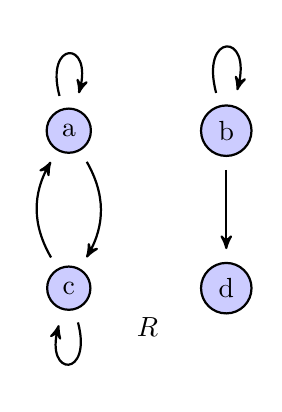
\begin{tikzpicture}[->,>=stealth',node distance=2cm,
                    thick,main node/.style={circle,fill=blue!20,draw,outer sep=5pt}
                   ]

  \node[main node] (a) {a};
  \node[main node] (b) [right of=a] {b};
  \node[main node] (c) [below of=a] {c};
  \node[main node] (d) [below of=b] {d};

  \path%
    (a) edge  [bend left] node {} (c)  %{} is where the edge value would go
        edge [loop above] node {} (a)
    (c) edge  [bend left] node {} (a)
         edge [loop below] node {} (c)
    (b) edge   node {} (d)  %{} is where the edge value would go
        edge [loop above] node {} (b);
   \node at (10mm,-25mm) {$R$};
\end{tikzpicture}
}\\[5pt]


\item Find the composition, $R\circ S$,  where $S = \{\,(1,a), (4,a),
(5,b), (2,c),  (3,c), (3,d)\,\}$ with $R  =\{(a,x),(a,y),(b,x),(c,z),(d,z)\}$ as a set of ordered pairs.\\[5pt]
{\color{blue} 
\[
R\circ S = \{ (1,x), (1,y), (4,x), (4,y), (5,x), (2,z), (3,z)\}
\]
}\\[5pt]

\item Let $R_1=\{(1,2), (1,3), (1,5), (2,1), (5,6), (6,6)\}$ and\\
$R_2=\{(1,2),(1,6), (3,6), (4,2), (5,6), (6,2), (6,3)\}$. Find $R_1\cup R_2$ and $R_1\cap R_2$. \\[5pt]

{\color{blue}
\[
R_1\cup R_2 = \{ (1,2), (1,3) , (1,5), (1,6), (2,1), (3,6), (4,2), (5,6).(6,2), (6,3), (6,6) \}
\]

\[
 R_1\cap R_2 = \{ (1,2), (5,6) \}
\]
}\\[5pt]

\item Define a relation on $\{1,2,3,4,5\}$ by $R=\{(1,2),(2,1),(2,3),(3,2),(3,4),(4,3),\\
(4,5),(5,4),(5,1),(1,5)\}$. For each of the five properties of a relation defined in this chapter 
(reflexive, irreflexive, symmetric, antisymmetric, and transitive) 
either show $R$ satisfies the property, or explain why it does not.
\\[5pt]

{\color{blue}
\begin{itemize}

\item \underbar{not reflexive}: $R$ is not reflexive since, for example, $(1,1)$ is not in $R$.\\[3pt]

\item \underbar{irreflexive}: Since $(1,1), (2,2), (3,3), (4,4), (5,5)$ are all missing from $R$, 
that means $R$ is irreflexive.\\[3pt]

\item\underbar{symmetric}: Since the reverse of each ordered pair in $R$ is also in $R$, $R$ is 
symmetric.\\[3pt]

\item\underbar{not antisymmetric}: Since $(1,2)$ and $(2,1)$ are both in $R$, but $1\not=2$, $R$
is not antisymmetric.\\[3pt]

\item\underbar{not transitive}: $(1,2)$ and $(2,3)$ are both in $R$, but $(1,3)$ is not in $R$, 
so $R$ is not transitive.\\[5pt]

\end{itemize}
}
\vfill\break

\item Define the relation {\it $M(A,B) : A\cap B \not= \emptyset$}, where the
domains for $A$ and $B$ are all subsets of $\mathbb{Z}$. For each of the five properties of a 
relation defined in this chapter (reflexive, irreflexive, symmetric, antisymmetric, and transitive) 
either show $M$ satisfies the property, or explain why it does not.
\vskip 4pt
Hint: This problem causes a lot of grief. The relation $M$ is a relation between \underbar{subsets} 
of $\mathbb{Z}$. For example, $\{1,2\} M \{ 9\}$ is false, since $\{1,2\}\cap \{9\} = \emptyset$. But 
$\{1,2\} M \{2,4,6,7\}$ is true since $\{1,2\} \cap \{2,4,6,7\} = \{2\}$, and not $\emptyset$.\\[5pt]
{\color{blue}
\begin{itemize}

\item \underbar{not reflexive}: $M$ is not reflexive since, for (the only!)  example, $\emptyset\,M\,\emptyset$ is false.\\[3pt]

\item \underbar{not irreflexive}: Since $\{1\}\,M\,\{1\}$ is true, 
that means $M$ is not irreflexive.\\[3pt]

\item\underbar{symmetric}: Since $A\cap B = B \cap A$, if $A\,M\,B$ is true, then $B\,M\,A$ is true. That shows $M$ is 
symmetric.\\[3pt]

\item\underbar{not antisymmetric}: Since $\{1\}\,M\,\{1,2\}$ and  $\{1, 2\}\,M\,\{1\}$ are both true, but 
 $\{1\} \not= \{1,2\}$, $M$ is not antisymmetric.\\[3pt]

\item\underbar{not transitive}: $\{1\}\,M\,\{1,2\}$ and $\{1,2\}\,M\,\{2\}$ are both true, but $\{1\}\,M\,\{2\}$
is false, 
so $M$ is not transitive.\\[5pt]

\end{itemize}
}

\vfill\break

\item (bonus)  Let $A=\emptyset$ and consider the empty relation, $E=\emptyset$,  on $A$. 
For each of the five properties of a 
relation defined in this chapter (reflexive, irreflexive, symmetric, antisymmetric, and transitive) 
either show $M$ satisfies the property, or explain why it does not.

\underbar{Warning}: Reasoning about the empty set can cause grave mental anguish. Suggestion: write out each of the
five definitions you need to check (reflexive, symmetric, etc.) and decide if the statement is true or false.

For example: For the reflexive condition, the statement to check is

\[
\forall x ( x\in \emptyset \implies (x,x)\in E)
\]

Since the left side of the implication ($x\in \emptyset$) is definitely false (after all there isn't anything in the empty set!)
the entire implication is true (recall the truth table for implication). That means the proposition above is true, and so $E$ is reflexive. Reasoning for the remaining four conditions all follow a similar pattern.\\[5pt]

{\color{blue}
The five propositions to check are:

\begin{itemize}

\item \underbar{reflexive}: $\forall x ( x\in \emptyset \implies (x,x)\in \emptyset)$\\[3pt]

\item \underbar{irreflexive}: $\forall x ( x\in \emptyset \implies (x,x)\not\in \emptyset)$\\[3pt]

\item\underbar{symmetric}: $\forall x \forall y( (x,y) \in \emptyset \implies (y,x)\in \emptyset)$\\[3pt]

\item\underbar{antisymmetric}: $\forall x\forall y ( ((x,y)\in \emptyset \land (y,x) \in \emptyset) \implies x=y)$\\[3pt]

\item\underbar{transitive}: $\forall x \forall y\forall z( ((x,y)\in \emptyset \land (y,z)\in \emptyset) \implies (x,z)\in \emptyset)$\\[5pt]

\end{itemize}

In every case, the condition to check has the form $p\implies q$, and the $p$ portion will be false, so the entire
entire predicate will always be true. That means $E$ has all five properties.
}

\end{enumerate}

\section{Lesson 6}

\begin{enumerate}

\item Let $A$ be the set of people alive on earth. 
For each relation defined below, determine if
it is an equivalence relation on $A$. {\bf If it is, describe the equivalence classes.}
If it is not, determine which properties of an equivalence relation fail.\\[3pt]

\begin{enumerate}

\item $a\,H\,b \iff$  $a$ and $b$ are the same age in (in years).\\[3pt]
{\color{blue}
$H$ is reflexive since everyone is the same age as themself.\\
$H$ is symmetric since if $a$ is the same age as $b$, then $b$ is the same age as $a$.\\
$H$ is transitive since if $a$ and $b$ are the same age, and $b$ and $c$ are the same age,
then $a$ and $c$ are the same age.\\
So, $H$ is an equivalence relation. An equivalence class will consist of all people of some one specific age. 
For example, one equivalence
class will be the set of all $38$ year old people.\\[3pt]
}

\item $a\,G\,b \iff$  $a$ and $b$ have grandparent in common.\\[3pt]
{\color{blue}
$G$ is reflexive since everyone has a grandparent in common with themself.\\
$G$ is symmetric since if $a$ has a grandparent in common with $b$, then $b$ has a grandparent in common with  $a$.\\
$G$ is not transitive: suppose $a$ has grandparents $(r,s)$ and $(t,u)$, and $b$ has grandparents 
$(t,u)$ and $(v,w)$  and $C$ has grandparents $(v,w)$ and $(x,y)$. Then $a\, G\, b$ and $b\,G\,c$ are both
true, but $a\,G\,c$ is false.\\
So $G$ is not an equivalence relation.\\[5pt]
}

\end{enumerate}

\item Consider the relation {\it $S(x,y) : x$ is a brother or sister of $y$} (or $x$ and $y$ are siblings) on the set, $H$,
of living humans. (Here {\it brother of} will mean a male with the same two parents, so don't consider {\it half brothers}. Likewise, don't consider {\itshape half siblings}.) Which of the three properties, reflexive, symmetric, transitive,
hold for the relation $S$? (Hint: Think carefully about transitive! Almost everyone gets this part wrong.) 
Is $S$ an  equivalence relation on $H$?\\[3pt]
{\color{blue}
$S$ is not reflexive since a person cannot be their own sibling. \\
$S$ is symmetric since if $a$ and $b$ are siblings, then $b$ and $a$ are siblings.\\
$S$ is not transitive. For example, Suppose $Bill$ and $Jill$ are brother and sister.\\
Then $Bill\,S\, Jill$ and $Jill\,S\,Bill$ are both true, but $Bill\,S\,Bill$ is false.\\
That shows $S$ is not transitive.\\[5pt]
}


\item  There are many different equivalence relation possible on the set $A=\{a,b,c,d\}$. For example,
here are just three different ones:\\[3pt]
\begin{enumerate} 
\item$E_{1} = \{(a,a), (b,b), (c,c), (d,d), (a,c), (c,a),(b,d),(d,b)\}.$\\[3pt]
\item$E_{2} = \{(a,a), (b,b), (c,c), (d,d), (a,c), (c,a),(a,b),(b,a),(b,c),(c,b)\}.$\\[3pt]
\item $E_{3} = \{(a,a), (b,b), (c,c), (d,d)\}.$\\[3pt]
\end{enumerate}

$E_{1}$ has $8$ ordered pairs while $E_{2}$ has $10$ and $E_{3}$ has $4$. Question: Of all the possible equivalence relations on $A$, what is the largest number of ordered pairs possible in the relation?\\[3pt]
{\color{blue}
The largest possible equivalence relation on $A$ would have all $16$ ordered pairs in $A\times A$.\\[5pt]
}


\item Let $A$ be the set of all ordered pairs of positive integers.
So some members of $A$ are $(3,6),  (7,7), (11,4), (1,2981)$. A relation on $A$ is defined by the rule 
$(a,b) R (c,d)$ if and only if $ad = bc$. For example $(3,5) R (6,10)$ is true since $(3)(10)=(5)(6)$.\\[3pt]
\begin{enumerate}
\item Explain why $R$ is an equivalence relation on $A$.\\[3pt]
{\color{blue}
reflexive: Is (a,b)R(a,b) true? Yes, since ab = ba.\\
symmetric: If (a,b)R(c,d) is true, is (c,d)R(a,b) true? Yes, since if
(a,b)R(c,d) is thrue, then ad = bc, So cb = da, and that means (c,d)R(a,b) is true.\\
Transitive: If (a,b)R(c,d) and (c,d)R(e,f) are true, is (a,b)R(e,f) true? Yes.\\
Suppose (a,b)R(c,d) and (c,d)R(e,f) are true. The ad = bc and cf = de. That
means (ad)(cf) = (bc)(de). Since the letters represent positive integers,\\
we can cancel c and d to get af = be. That means (a,b)R(e,f) is true.\\[3pt]
}

\item List four ordered pairs in the equivalence class of $(2,3)$.\\[3pt] 
{\color{blue}
Any ordered pair of positive integers, $(a,b)$ with $3a=2b$ will do.\\
 Examples:
$(2,3), (4,6), (6,9), (8,12)$.\\[5pt]
}
\end{enumerate}


\item   Let $A=\{1,2,3,4,5,6\}$. 
Form a partition of $A$ using $\{1, 2\}, \{3, 4, 5\}$, and $\{6\}$.
These are the equivalence classes for an equivalence relation, $E$, on $A$.
 Draw the  {\bf digraph} of $E$.\\[3pt]
 
 {\color{blue}
 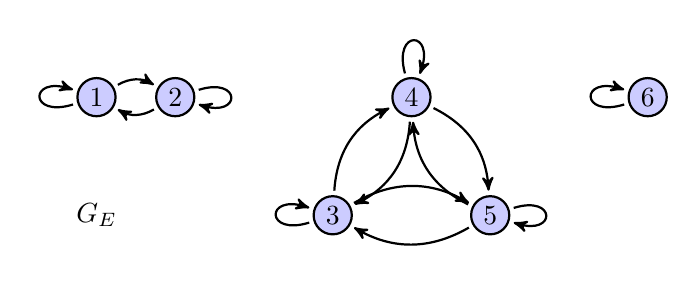
\begin{tikzpicture}[->,>=stealth',node distance=2cm,
                       thick,main node/.style={circle,fill=blue!20,draw,outer sep=2pt,inner sep=2pt}
                      ]

  \node[main node] (1) at (-2.0,1.5) {$1$};
  \node[main node] (2) at (-1.0,1.5) {$2$};
  \node[main node] (3) at (1.0,0.0) {$3$};
  \node[main node] (4) at (2.0,1.5) {$4$};
  \node[main node] (5) at (3.0,0.00) {$5$};
  \node[main node] (6) at (5.0,1.5) {$6$};
  \node (E) at (-2.0,0.0) {$G_E$};
  
  \path%
   (1) edge  [out=197.5,in=162.5,looseness=8] node {} (1)
        edge [bend left,->] node {} (2)
   (2) edge  [out=17.5,in=-17.5,looseness=8] node {} (2)
        edge [bend left] node {} (1);

 a a \path%
   (3) edge [out=197.5,in=162.5,looseness=8] node {} (3)
        edge [bend left] node {} (4)
        edge [bend left] node {} (5)
   (4) edge [out=105.5,in=70.5,looseness=8] node {} (4)
        edge [bend left] node {} (3)
        edge [bend left] node {} (5)
   (5) edge [out=17.5,in=-17.5,looseness=8] node {} (5)
        edge [bend left] node {} (3)
        edge [bend left] node {} (4);
  \path%
  (6) edge [out=197.5,in=162.5,looseness=8] node {} (6);
   \end{tikzpicture}
}

\vskip 5pt 

\item (bonus) Let $A = \{ 1,2,3\}$. The relation $E = \{ (1,1),(2,2),(3,3),(2,3),(3,2)\}$ is an
equivalence relation on $A$.  $F=\{ (1,1),(2,2),(3,3),(1,2),(2,1)\}$ 
is another equivalence relation on $A$. Compute the composition $F\circ E$.
Is $F\circ E$ and equivalence relation on $A$?\\[3pt]

{\color{blue}
$F\circ E =  \{(1,1), (1,2), (2,1), (2,2), (2,3), (3,1), (3,2), (3,3)\}$.

$F\circ E$ is not symmetric since $(3,1)$ is in $F \circ E$, but $(1,3)$ is not.

$F \circ E$ is not transitive since $(1,2)$ and $(2,3)$ are in $F\circ E$ but $(1,3)$ is not.

So, $F\circ E$ is not an equivalence relation on $A = \{1,2,3\}$.\\[5pt]
}


\end{enumerate}

\vfill\break

\section{Lesson 7: Test \#1}

Part I:  ($2\frac{1}{2}$ points each) \underbar{True or False} (circle your answer): 

\vskip 10pt
\begin{enumerate}
\item {\bf {\color{red}True} \ \  False}: The following sentence is a proposition: {\itshape The earth is flat.} 

\vfill

\item  {\bf {\color{red}True} \ \  False}: $\neg(p\longrightarrow q) \equiv p\land\neg q$

\vfill
 
 \item  {\bf True \ \  {\color{red}False}}: $\exists{x}\forall{y} P(x,y) \equiv \forall{y}\exists{x}P(x,y)$ 
 
\vfill
  
\item  {\bf {\color{red}True} \ \  False}: $s\longrightarrow t\, {\it and }\,   \neg t, \quad \therefore \neg s$ is a valid rule of inference. 

\vfill

\item  {\bf True \ \ {\color{red} False}}: There is an element of the empty set bigger than $2$.
 
 \vfill
 
\item  {\bf {\color{red}True} \ \  False}: The set $\{\,1,\, \{1,2\},\, \{2\}\,\}$ has three elements.

\vfill
 
\item  {\bf {\color{red}True} \ \  False}: For all sets $A,B$, we have  $A\cap B\subseteq A\cup B$.

\vfill
 
\item  {\bf True \ \ {\color{red} False}}: In a direct proof of $H\longrightarrow C$ it is OK to use $\neg C$ as a step. 
  
\vfill
  
\item  {\bf {\color{red}True} \ \  False}: $cat\,C\,t$ is true for the  relation  $C(x,y)$: {\it the word $x$ uses letter $y$}.
 
 \vfill
 
\item  {\bf {\color{red}True} \ \  False}: The relation on the set of all people 
\vskip -1pt\hskip 70pt $S(x,y)$: {\it $x$ and  $y$ are the same age}
\vskip -1pt\hskip 70pt is transitive.

\vfill

\item  {\bf {\color{red}True}\ \  False}: The smallest counterexample to the proposition
 \vskip -1pt\hskip 70pt {\it For every positive integer $n$, the number $n^2+n+1$ is a prime} 
\vskip -1pt\hskip 70pt  is $n=4.$\vfill

\item {\bf True \ \ {\color{red} False}}: The relation $G(x,y)$ {\it x has met y} is an equivalence
\vskip -1pt\hskip 70pt relation on the set of all people.
 
 \end{enumerate}
 \vfill
 \break
 
 
 
 
 
II: (5 points each) \underbar{Multiple Choice} (circle your answer):

\vfill

1) The converse of $u\longrightarrow v$ is

\hskip 20pt {\color{red}(a) $v \longrightarrow u$}\hfill

\hskip 20pt (b) $\neg v \longrightarrow u$\hfill

\hskip 20pt (c) $\neg u \longrightarrow v$\hfill

\hskip 20pt (d) $\neg v \longrightarrow \neg u$\hfill

\hskip 20pt (e) none of the above\hfill

\vfill


2) $\neg \exists{x}\forall{y}\,P(x,y)$ is logically equivalent to

\vskip 5pt
\hskip 20pt (a) $ \forall{x}\exists{y}\,\neg P(y,x)$\hfill
\vskip 5pt
\hskip 20pt (b) $\exists{y}\forall{x}\,P(x,y)$\hfill
\vskip 5pt
\hskip 20pt (c) $\exists{x}\forall{y}\,\neg P(x,y) $\hfill
\vskip 5pt
\hskip 20pt {\color{red}(d) $\forall{x}\exists{y}\,\neg P(x,y)$}\hfill
\vskip 5pt
\hskip 20pt (e) $\forall{x}\neg \exists{y}\,P(x,y)$\hfill

\vfill

3)  If the set $A\times B$ has $45$ elements and the set $A$ has $5$ elements, then the
number
\vskip -1pt\hskip 13pt  of elements in $B$ is

\vskip 5pt
\hskip 20pt (a) $4$\hfill
\vskip 5pt
\hskip 20pt{\color{red} (b) $9$}\hfill
\vskip 5pt
\hskip 20pt (c) $25$\hfill
\vskip 5pt
\hskip 20pt (d) $40$\hfill
\vskip 5pt
\hskip 20pt (e) $45$\hfill

 
\vfill


4) The first line in a proof of {\bf THM}: {\it If $B$ is a  blisk, then $B$ is a glumx.} is 
\vskip -1pt\hskip 13pt {\it Suppose  $B$ is a blisk, and $B$ is not a glumx.}
The method of proof being used is:

\vskip 5pt
    \hskip 20pt {\color{red}(a) Proof by Contradiction}\hfill
\vskip 5pt
\hskip 20pt (b) Direct Proof\hfill
\vskip 5pt
\hskip 20pt (c) Indirect Proof\hfill
\vskip 5pt
\hskip 20pt (d) Proof by Cases\hfill
\vskip 5pt
\hskip 20pt (e) Proof by Confusion\hfill

\vfill
\break

5)  $R$ is the relation on the integers given by {\itshape $R(n,m)$: $n+m$ ends with $0$}. For example,
\vskip -1pt\hskip 13pt $R(18,102)$ is true since $18+102 = 120$, and $120$ does end with a $0$. But $55+11= 66$
\vskip -1pt\hskip 13pt so $R(55,11)$ is false since $66$ does not end with a $0$. Circle all the  
properties the  relation 
\vskip -1pt\hskip 13pt $R$ has in the list below.

\vskip 5pt
\hskip 20pt (a) Reflexive\hfill
\vskip 5pt
\hskip 20pt {\color{red}(b) Symmetric}\hfill
\vskip 5pt
\hskip 20pt (c) Antisymmetric\hfill
\vskip 5pt
\hskip 20pt (d) Transitive\hfill
\vskip 5pt
\hskip 20pt (e) $R$ has none of those four properties.\hfill

\vfill

6) Let $R$ be the relation from $\{1,2,3,4\}$ to $\{x,y\}$ given by $R=\{(1,x), (1,y),(2,x),(3,y),(4,x)\}$\vskip -1pt\hskip 13pt  and let $S$ be the relation from $\{x,y\}$ to $\{a,b,c\}$
given by $S = \{(x,a),(x,c),(y,b)\}.$\vskip -1pt\hskip 13pt 
 Circle all the ordered pairs that are in $S\circ R$.  


\vskip 4pt
\hskip 20pt {\color{red}(a) $(1,b)$}\hfill
\vskip 4pt
\hskip 20pt {\color{red}(b) $(2,c)$}\hfill
\vskip 4pt
\hskip 20pt (c) $(b,4)$\hfill
\vskip 4pt
\hskip 20pt (d) $(a,1)$\hfill
\vskip 4pt
\hskip 20pt (e) $(x,y)$\hfill

\vfill

7) Let  $A =\{ 1,2,3,4\}$ and let $B=\{2,4,6,8\}$. Circle all the  
true statements in the list below.

\vskip 3pt
\hskip 20pt {\color{red}(a) $2\in A\cap B$}\hfill
\vskip 3pt
\hskip 20pt{\color{red}(b) $(2,2)\in A\times B$}\hfill
\vskip 3pt
\hskip 20pt (c) $2\in A-B$\hfill
\vskip 3pt
\hskip 20pt {\color{red}(d) $2\in A\cup B$} \hfill
\vskip 3pt
\hskip 20pt {\color{red}(e) $(2,2)\in B\times A$} \hfill

\vfill

8) Let $C$ be the relation on the cards in the usual $52$ card deck defined by 
$C(x,y)$: {\it $x$ and 
\vskip -1pt\hskip 13pt $y$ have the same suit}. Circle all the  
true statements in the list below.

\vskip 3pt
\hskip 20pt {\color{red}(a) The equivalence class, $[3\spadesuit]$, of the $3\spadesuit$ contains $13$ elements.}\hfill
\vskip 3pt
\hskip 20pt (b) The equivalence class, $[3\spadesuit]$, of the $3\spadesuit$ contains $4$ elements.\hfill
\vskip 3pt
\hskip 20pt {\color{red}(c) $[3\spadesuit]=[4\spadesuit]$.}\hfill
\vskip 3pt
\hskip 20pt (d) $[3\spadesuit]=[3\clubsuit]$ \hfill
\vskip 3pt
\hskip 20pt (e) None of the above statements are true.\hfill

\vfill
\break

III. ($10$ points each) \underbar{Problems} 

\underbar{\small Do any three of the following four problems. If you do all four, I'll count your best three.}


1) Use a truth table to determine if $\lnot p \lor (q\to r)$ is logically 
equivalent to $\lnot r\lor (p\to \lnot q)$.\\[3pt]

{\color{blue}
\begin{tabular}{c  c  c |  c | c}
$p$ & $q$ & $r$ &    $\lnot p \lor(q \to r)$ &  $\lnot r\lor (p\to \lnot q)$ \\
\hline
T & T & T &   T &   F  \\
T & T & F &   F &   T \\
T & F & T &   T &    T  \\
T & F & F &   T &  T  \\
F & T & T &   T &  T  \\
F & T & F &   T &  T  \\
F & F & T &   T &  T  \\
F & F & F &   T &  T  \\
\end{tabular}\\[3pt]

Since the truth table for the two propositions do not match in at least one row, the two propositions are not
logically equivalent.\\[5pt]
}

\vfill

2) Express the following argument in symbolic form and show, {\bf by applying rules of inference}, that
the argument is valid. Give the reason for each step in your proof.\\[3pt]


{\itshape If it is either Monday or Tuesday, then  classes are cancelled.  If classes are cancelled, the exam will be postponed. 
The exam is not postponed. So, it is not Monday. }\\[3pt]

{\color{blue}
Let $m$ be {\itshape It is Monday}, $t$:{\itshape It is Tuesday}, $c$: {\itshape Classes are cancelled}, $e$: {\itshape The exam is postponed}.\\[2pt]

The argument:

\begin{tabular}[t]{l}
   $(m\lor t) \to c$\\
   $c \to e$\\
   $\lnot e$\\
   \vrule width .75in depth 0pt height .5pt\\
   so: $\lnot m$
   \end{tabular}
 \qquad\textbf{Proof:}
 \begin{tabular}[t]{r l l}
 (1)& $c\to e$                   & hypothesis\\
 (2)& $\lnot e$      & hypothesis\\
 (3)& $\lnot c$                   & Modus Tolens (1) and (2)\\
 (4)& $(m\lor t) \to c$ & hypothesis\\
 (5)& $\lnot(m \lor t)$ & Modus Tolens (3) and (5)\\
 (6)& $\lnot m \land \lnot t$     & De Morgan's Law\\      
 (7)& $\lnot m$             & Simplification\\
 \end{tabular}\\[5pt]
}


\vfill
\break

3) Give a direct proof that the product of an even integer and an odd integer is even. \\[3pt]
{\color{blue}
Suppose $m$ is an even integer and $n$ is an odd integer. That means $m = 2j$ and $n = 2k+1$ for some integers $j$ and $k$. So, $mn = (2j)(2k+1) = 2(2jk+j)$. Since $2jk+j$ is an integer, that shows $mn$ is even.\\[5pt]
}

\vfill

4) Let $D=\{\, 1, 2, 3, 4, 5, 6, 7, 8, 9\,\}$, the set of nonzero digits. Let $S$ be the
relation on $D$ defined by $S(x,y)$: {\it The (English) names of $x$ and $y$ start with the same letter}. Explain why $S$ is an equivalence relation on $D$ and list the elements of the
equivalence class of $2$.\\[3pt]
{\color{blue} 
$S$ is reflexive since each digit has the same initial letter in its name as itself. $S$ is symmetric since if digits $m$ and $n$ have names starting with the same letter, so do $n$ and $m$. $S$ is transitive since if the names of $m$ and $n$ start with the same letter, and the names of $n$ and $t$ start with the same letter, then the names of $m$ and $t$ start with the same letter. That shows $S$ is an equivalence relation on $D$. The equivalence class of $2$ will the the digits in $D$ with name starting with the letter $t$. So, $[2] = \{2,3\}$.\\[5pt]}

\vfill
\section{Lesson 8}

\begin{enumerate}

\item  What is the $50^{th}$ term of the arithmetic sequence with initial
term $4$ and common\\
 difference $3$?\\[3pt]
 {\color{blue}
 The $50^{th}$ term is $4 + (49)(3) = 151$.\\[5pt]
 }


\item Evaluate $\displaystyle\sum_{k=-3}^{4} (2k+5)$. (Hint: Since there are only eight terms in the sum, you can just write
them all out and add.)\\[3pt]
{\color{blue}
\[
\sum_{k=-3}^{4} (2k+5) = -1+1+3+5+7+9+11+13=48.\\[5pt]
\]
}

\item   Evaluate $\displaystyle \sum_{i=0}^{99} \left(-\frac{2}{3}\right)^i$. (Hint: Since there are $100$ terms in the sum, it isn't a good idea to write them all out and add. Use the formula for the sum of terms of a geometric sequence. Leave the answer with exponents rather than using a calculator to try to get a decimal approximation of the answer.) \\[3pt]
{\color{blue}
\[
\sum_{i=0}^{99} \left(-\frac{2}{3}\right)^i = \frac{ 1 - \left(-\frac{2}{3}\right)^{100}}{1-\left(-\frac{2}{3}\right)}
= \frac{3^{100}-2^{100}}{5\cdot 3^{99}}\\[5pt]
\]
}

\item 
\begin{enumerate}

\item List the first four terms of the sequence defined recursively by
 $a_0 = 2$, and, for $n\geq 1$, $a_n = 2a_{n-1}^2 -1$.\\[3pt]
 
 {\color{blue} $2, 7, 97, 18817$\\[5pt]}

\item List the first five terms of the sequence with initial terms
$u_1=1$ and $u_2=5$, and, for $n\geq 3$, $u_n = 5u_{n-1}-6u_{n-2}$.
Guess a closed form formula for the sequence.
Hint: The terms
are simple combinations of powers of $2$ and powers of $3$.\\[3pt]

{\color{blue} $1, 5, 19, 65, 211$. Closed form formula: $u_n = 3^n - 2^n$.\\[5pt]}


\end{enumerate}

\item  Give a {\bf recursive} definition of the geometric sequence
with initial term $a$ and common\\
 ratio $r$. 

Hint: $a_{n} = a r^{n-1}$ isn't a correct answer since this formula isn't recursive.
Make sure you write down a recursive formula: (1) give the initial term, and 
(2) give the rule for building new terms from previous terms.\\[3pt]

{\color{blue} $a_0 = a$ and, for $n\geq 1$, $a_n = ra_{n-1}$\\[5pt] }

\item (bonus) Express in summation notation: $\displaystyle  \frac{1}{1}+\frac{1}{3}+\frac{1}{5}+
\cdots+\frac{1}{2n-1}$, the sum of the reciprocals of the first $n$ odd
positive integers. (Note that there are $n$ terms in the sum.)

Hint: A common mistake on this question is using the symbol $n$ both as an index for summation
and to indicate the last term to be added in. To make sure you haven't fallen into that trap, replace every
$n$ in your formula by a specific value, say $5$. The result should be a sum
  $\displaystyle  \frac{1}{1}+\frac{1}{3}+\frac{1}{5}+\frac{1}{7}+\frac{1}{9}$.\\[3pt]
  {\color{blue}
  \[ 
  \sum_{k = 1}^n \frac{1}{2k-1}\\[5pt]
  \]
  }

 \end{enumerate}
 
 \section{Lesson 9}
 
 \begin{enumerate}
 
 \item A set $S$ of integers is defined recursively by the rules: \\[2pt]
 (1) $1\in S$, and (2) If $n\in S$, then
 $2n+1 \in S$. \\[2pt]
 
 \begin{enumerate} 
 \item Is $20\in S$?\\[2pt]
 \item Is $175\in S$?\\[2pt]
 
 {\color{blue} The   smallest elements of $S$ are $1, 3, 7, 15, 31, 63, 127, 255$.
 So neither $20$ nor $175$ is in $S$.\\[5pt]}
 
 \end{enumerate}
 Explain your answers.\\[5pt]
 
 \item A set, $S$, of strings over the alphabet 
$\Sigma = \{a,b,c\}$ is defined recursively by (1) $a \in S$
and (2) if $x\in S$ then $xbc\in S$. List all the strings in $S$ of length seven or less.\\[3pt]

{\color{blue} $a, abc, abcbc, abcbcbc$\\[5pt]}


\item A set, $S$, of positive integers is defined recursively by the rule:\\[2pt]
(1) $3\in S$, and (2) If $n\in S$, then $2n-3\in S$. List {\bfseries all} the elements in the set $S$.\\[3pt]

{\color{blue} $S = \{3\}$\\[5pt]}
 
 \item Give a recursive definition of the set of positive integers that end with the digit $7$.\\[3pt]
 
 {\color{blue} (1) $7\in S$, and, (2) if $n\in S$, then $n+10\in S$.\\[5pt]}

 
\item Describe the strings in the set $S$ of strings over the alphabet 
$\Sigma = \{a,b,c\}$ defined recursively by (1) $ c \in S$
and (2) if $x\in S$ then $xa\in S$ and $xb\in S$ and $cx\in S$.\\[3pt]

Hint: Your description should be a sentence that provides an easy test to check if a given string
is in the set or not. An example of such a description is: {\it $S$ consists of all strings of $a$'s, $b$'s, and $c$'s,
with more $a$'s than $b$}'s. That isn't a correct description since $cab$ is in $S$ and doesn't have more $a$'s than
$b$'s, and also $baac$ isn't in $S$, but does have more $a$'s than $b$'s. So that attempted description is really 
terrible. The best way to do this problem is to use the rules to build a bunch of strings in $S$ until a suitable
description becomes obvious.\\[3pt]

{\color{blue} The strings in $S$ have the form one or more $c$'s followed on the right by any
string of zero or more $a$'s and $b$'s.\\[5pt]}

\item (bonus)  A set $S$ of ordered pairs of integers is defined recursively
by (1) $(1,2)\in S$  and $(2,1)\in S$,  and (2) if $(m,n)\in S$, then $(m+2,n)\in S$, and
$(m,n+2)\in S$, and $(m+1,n+1)\in S$. There is a simple description
of the ordered pairs in $S$. What is it?  Your description should be good enough so that 
you can instantly decide if $(12236, 912242)$ is in $S$. \\[3pt]

{\color{blue} $S$ is the set of all ordered pairs of positive integer 
that have one coordinate even and the other coordinate odd.\\[5pt]}


\end{enumerate}

\section{Lesson 10}

\begin{enumerate}

\item[]
{\small {\bf Warning}: It's not unusual to find these problems really tough. One difficulty is that these problems will make some demands on your algebra skills. Another difficulty is just getting the format of an inductive proof correct.  Here are a few suggestions concerning that: (1)
Be sure to check the basis case; (2) At the start of the inductive step, clearly state the inductive hypothesis;
(3) After stating the inductive hypothesis, write down what you need to prove; (4) Point out clearly where you
apply the inductive hypothesis in the proof of the inductive step.}\\[3pt] 


\item Use induction to prove: For every integer $n\geq 1$,
\[
1\cdot 2+ 2\cdot 3+3\cdot4+\cdots+n(n+1) = \frac{n(n+1)(n+2)}{3}.\\[3pt]
\]
{\color{blue}
\underbar{Basis}: For $n=1$, the left side of the equation is $1\cdot 2 = 2$ and the right side is
$\frac{(1)(2)(3)}{3} = 2$, so the equality is correct for this case.\\[2pt]
\underbar{Inductive Step}:\\ Suppose  $\displaystyle 1\cdot 2+ 2\cdot 3+3\cdot4+\cdots+n(n+1) = \frac{n(n+1)(n+2)}{3}$ for some $n\geq 1$. Then
\begin{align*}
1\cdot 2+ 2\cdot 3+3\cdot4+&\cdots+n(n+1) +(n+1)(n+2)\\[2pt]
&= \frac{n(n+1)(n+2)}{3} +(n+1)(n+2)\\[2pt]
& = \frac{n(n+1)(n+2)}{3} +\frac{3(n+1)(n+2)}{3}\\[2pt] 
& = \frac{n(n+1)(n+2) +3(n+1)(n+2)}{3}\\[2pt]
& = \frac{(n+1)(n+2)(n+3)}{3}.\clubsuit\\[5pt]
\end{align*}
}


\item  Use the first form of induction (see example 16.5) to show that using only $4 c\kern -5pt/$ stamps and  $7c\kern -5pt/$ stamps,
any postage amount $18c\kern -5pt/$ or greater can be formed.\\[3pt]
{\color{blue}
\underbar{Basis}: We can make $18c\kern -5pt/$ using two $7c\kern -5pt/$ and one $4c\kern -5pt/$ stamps.\\[2pt]
\underbar{Inductive Step}: Suppose we can make $n c\kern -5pt/$ postage for some $n\geq 18$.
In that $n c\kern -5pt/$ postage there must be  at least five $4c\kern -5pt/$ stamps or at least one $7c\kern -5pt/$ stamp since otherwise the total would be at most $16c\kern -5pt/$.\\[2pt]
If there are five or more $4c\kern -5pt/$ stamps, remove five of them and put in three $7c\kern -5pt/$ stamps raising the total to $(n+1)c\kern -5pt/$. Otherwise,
remove one $7c\kern -5pt/$ and put in two $4c\kern -5pt/$ stamps, again raising the total to $(n+1)c\kern -5pt/$. So, in any case,  we can make $(n+1)c\kern -5pt/$ postage. $\clubsuit$\\[5pt]
} 


\item  Redo the previous problem using the second form of induction (see example in the text). The basis step is just a bit messier this time, but the inductive step is much easier.\\[3pt]

{\color{blue}
\underbar{Basis}: There are four cases in the basis step:\\
$18c\kern -5pt/$: one $4 c\kern -5pt/$ stamp and two  $7c\kern -5pt/$ stamps \\
$19c\kern -5pt/$: three $4 c\kern -5pt/$ stamps and one $7c\kern -5pt/$ stamp\\
$20c\kern -5pt/$: five $4 c\kern -5pt/$ stamps \\
$21c\kern -5pt/$: three $7c\kern -5pt/$ stamps \\[3pt]

\underbar{Inductive Step}: Suppose we can make all postage amounts from $18c\kern -5pt/$ up to some
$nc\kern -5pt/$ where $n\geq 21$. Then we can make $(n-3)c\kern -5pt/$ postage since $n-3$ is at least $18$
and less than $k$. Adding a $4 c\kern -5pt/$ stamp to the $(n-3)c\kern -5pt/$ postage gives us $(n+1)c\kern -5pt/$
postage. So, by induction, we can make all postage amounts $18c\kern -5pt/$ and greater. $\clubsuit$\\[5pt]
}

\item A sequence is defined recursively by the rules: (1) $a_{0} = 0$, and (2) for $n\geq 1$, $a_{n}= 2a_{n-1}+ 2$. Use induction to prove $a_{n}= 2^{n+1}-2$ for all $n\geq 0$.\\[3pt]
{\color{blue}
\underbar{Basis}: $a_{0}=0$ and $2^{0+1}-2 = 0$, so the formula $a_{n}= 2^{n+1}-2$ is correct for $n =0$.

\underbar{Inductive Step}: Suppose $a_{n}= 2^{n+1}-2$ is correct for some $n\geq 0$. Then\\
\[
a_{n+1} = 2a_{n}+2 = 2(2^{n+1}-2) + 2 = 2^{n+2} - 4 +2 = 2^{n+2} - 2
\]
as we needed to show.$\clubsuit$\\[5pt]
}

\item Use induction to prove: For every integer $n\geq 1$, the number $n^5-n$ is a multiple of $5$.

Hint: An integer is a multiple of $5$ if it is $5$ times some integer. For example,
$165 = (5)(33)$ so $165$ is a multiple of $5$.\\[3pt]

{\color{blue}
\underbar{Basis}: For  $n=1$  we have  $1^5 - 1 = 0 = (5)(0)$ is a multiple of
 $5$.\\
\underbar{Inductive Step}: Suppose  $n^5-n$ 
is a multiple of $5$ for some $n\geq 1$.
Then 
\begin{align*} 
(n+1)^5 - (n+1) &= (n^5 +5n^4 +10n^3+10n^2+5n+1) - n - 1\\
&= (n^5 - n) + 5(n^4  +2n^3+2n^2+n).
\end{align*}
The first group, $(n^5-n)$ 
 is a multiple of $5$ by the inductive hypothesis
and the second group has a factor of $5$ also. So
$(n+1)^5 - (n+1)$  is a multiple of $5$. $\clubsuit$\\[5pt]
}

\item   (bonus) Here is a {\itshape proof} that for $n\geq 0$,  $1+ 2 + 2^2 +  \cdots + 2^n = 2^{n+1}$.
\begin{proof}
Suppose $1+ 2 + 2^2 +  \cdots + 2^n = 2^{n+1}$ for some $n\geq 0$. Then
\begin{align*}
 1+ 2 &+ 2^2 +  \cdots + 2^n  + 2^{n+1} = 2^{n+1} +2^{n+1} \qquad\text{using the inductive hypothesis}\\
 &= 2(2^{n+1}) = 2^{n+2} = 2^{(n+1)+1},
 \end{align*}
 as we needed to show.
 \end{proof}
 
 Now, obviously there is something wrong with this proof by induction since, for example,
 $1+2+2^2 = 7$, but $2^{2+1} = 2^3 = 8$. What specifically is wrong with the proof?\\[3pt]
 {\color{blue}
 The error is that the basis case was not checked, and the basis case is not true
 since $1$ does not equal $2^{0+1}$.\\[5pt]
}

\end{enumerate}

\section{Lesson 11}

\begin{enumerate}

\item[]
{\small For the proofs requested below, use facts and theorem 
given in this lesson, including results given in the exercises,  as justifications. Assume all letters represent
integers.}\\[5pt]

\item  Mimic the proof given in the sample solutions for the proposition
 {\it if $a>0$ and $b>0$, then $ab>0$} to prove:\\[3pt]
 
\begin{enumerate}
\item If $a<0$ and $b<0$, then $ab>0$.\\[3pt]
{\color{blue} 
Suppose $a<0$ and $b<0$ are integers. Since $a<0$, multiplying both sides of $b<0$ by $a$ gives
$ab>a0$. We know $a0 = 0$. So $ab >0$. $\clubsuit$\\[5pt]
}

\item If $a<0$ and $b>0$, then $ab<0$.\\[3pt]
{\color{blue} 
Suppose $a<0$ and $b>0$ are integers. Since $a<0$, multiplying both sides of $b>0$ by $a$ given
$ab<a0$. We know $a0 = 0$. So $ab <0$. $\clubsuit$\\[5pt]
}

\end{enumerate}


\item 
Prove that is $m^{2} = n^{2}$, then $m=n$ or $m = -n$.\\
 (Hints: (1) From algebra: $a^{2}-b^{2} = (a+b)(a-b)$, and \\
 (2) From exercises: If $ab=0$, then either $a=0$ or $b=0$.) \\[3pt]
 
 {\color{blue}
 Suppose $m$ and $n$ are integers, and that $m^2 = n^2$. Then $m^2 - n^2 = 0$, and so $(m-n)(m+n) = 0$.
 In an exercise it was proved that if the product of two integers is $0$, then one or the other of the integers must be $0$.
 So, $m-n=0$ or $m+n=0$. That means $m=n$ or $m=-n$. $\clubsuit$\\[5pt]
 }

\item  Determine all the integers that $0$ divides.

Hint: Think carefully about the {\bf definition} of the {\it divides} relation! This question is about the divides relation, not about the arithmetic operation of division (a maybe subtle distinction). The correct answer is probably not what you might first think it is.\\[3pt]

{\color{blue}
Using the definition of divides,  {\it $0$ divides $0$} is true since $(0)(1) = 0$. If $n$ is not $0$, then $(0)(k)= 0\not= n$  for any integer $k$, so $0$ does not divide $n$. Conclusion: $0$ divides $0$, but no other integer.\\[5pt]
}


\item Prove: For integers $r,s,t$,and $u$, if $r|t$ and $s|u$, then $rs|tu$.\\[3pt]

{\color{blue} Suppose $r,s,t$,and $u$ are integers, and that $r|t$ and $s|u$. That means there are integers $a$ and $b$
such that $ar =t$ and $sb=u$. It follows that $(ar)(sb) = tu$. We can rearrange that as $(rs)(ab) = tu$, and since $ab$
is an integer, that shows $rs|tu$. $\clubsuit$\\[5pt]
}

\item Determine the quotient and remainder when $117653$ is
divided by $27869$. (Finally, an easy problem.)\\[3pt]

{\color{blue}
quotient is $4$\\
remainder is $6177$\\[5pt]
} 

\item (bonus) Prove or give a counterexample: If $p$ is a prime, then $6p+1$ is a prime.\\[3pt]

{\color{blue} Counterexample: For the prime $19$, the integer $6\cdot 19 + 1 = 115 = 5\cdot 23$ is not a prime.\\[5pt]
}
\end{enumerate}


\section{Lesson 12}

\begin{enumerate}

\item Use the Euclidean Algorithm to compute the following gcd's:\\[3pt]
 \begin{enumerate}
 \item $\gcd(216,111)$.
 {\color{blue}
 \begin{align*}
 216 &= 1\cdot111+105 \\
 111 &= 1\cdot105+6 \\
  105 &= 17\cdot6+3 \\
  6 &= 2\cdot3+0 \\
\end{align*}
$\gcd(216,111) = 3$\\[3pt]

 }
 \item $\gcd(1001,11)$.
 {\color{blue}
 \begin{align*}
 1001 &= 91\cdot11+0 \\
\end{align*}
$\gcd(1001,11) = 11$\\[3pt]

 }
 
 \item $\gcd(663,5168)$.
 {\color{blue}
 \begin{align*}
 5168 &= 7\cdot663+527 \\
 663 &= 1\cdot527+136 \\
  527 &= 3\cdot136+119\\
  136 &= 1\cdot119+17 \\
  119  &= 7\cdot17+0 \\
\end{align*}
$\gcd(663,5168) = 17$\\[3pt]
 }
 
 \item $\gcd(1357,2468)$.
{\color{blue}
 \begin{align*}
 2468 &= 1\cdot1357+1111 \\
 1357 &= 1\cdot1111+246 \\
  1111 &= 4\cdot246+127\\
  246 &= 1\cdot127+119\\
  127  &= 1\cdot119+8 \\
  119  &=14\cdot8+7\\
  8 &= 1\cdot 7 +1\\
  7 &= 7\cdot 1 + 0
\end{align*}
$\gcd(1357,2468) =1$\\[3pt]

 } 
 
 \item $\gcd(733103,91637)$.
 {\color{blue}
 \begin{align*}
 733103 &= 8\cdot91637 + 7\\
 91637 &= 13091\cdot7+0 
 \end{align*}
$\gcd(733013,91637) = 7$\\[5pt]

 }
 
  \end{enumerate}
 
 
\item  If $p$ is a prime, and $n$ is any integer, what are the
possible values of $\gcd(p,n)$?
Hint: Try a few experiments with specific numbers to spot the correct answer. Alternatively, think about the positive integers that can divide a prime. Warning: In the notation $\gcd(a,b)$, do not assume that $a\geq b$.
The two parameters $a$ and $b$ can be written in either order: $\gcd(15,12) = \gcd(12,15) = 3$.\\[3pt]
{\color{blue}
Since the only positive divisors of a prime $p$ are $1$ and $p$, those are the only two possible values of $\gcd(p,n)$. In fact, $\gcd(p,n) = 1$ if $p$ does not divide $n$ and $\gcd(p,n) = p$ if $p$ does divide $n$.\\[5pt]
}


\item Determine $\gcd(6123,2913)$ and write it as a linear combination of $6123$ and $2913$. 

{\color{blue}

\begin{table}[!h]
\renewcommand{\arraystretch}{1.25}
\begin{tabular}{|*{9}{>{\raggedleft\arraybackslash}p{0.996cm}|}}
 \hline
 6123&2913&297&240&57&12&9&3&0\\
  \hline
  &&2&9&4&4&4&1&3 \\
 \hline
 0&1&-2&19&-21&103&-433&536&-2041 \\
 \hline
 1&0&1&-9&10&-49&206&-255&981 \\
 \hline
\end{tabular}
\end{table}

Thus, we may conclude that 
\[
\gcd(6123,2913) = 3 = (6123)(-255) + (2913)(536).\\[5pt]
\]

}

\item What can you conclude about $\gcd(a,b)$ if there are integers $s,t$ such that $as+bt = 8$?\\[3pt]
{\color{blue}
Since the linear combinations of $a$ and $b$ are the multiples of $\gcd(a,b)$, it must be the case that
$\gcd(a,b)$ must be a positive divisor of $8$. In other words, $\gcd(a,b) = 1, 2, 4,$ or $8$.\\[5pt] 
}

\item What is the smallest positive integer that can be written as a linear combination of $2191$ and  $1351$?\\[3pt]
{\color{blue}
The answer is the gcd of $2191$ and $1351$.
 \begin{align*}
 2191 &= 1\cdot1351+840 \\
 1351 &= 1\cdot840+511 \\
  840 &= 1\cdot511+329\\
  511 &= 1\cdot329+182\\
  329  &= 1\cdot182+147 \\
  182  &=1\cdot147+35\\
  147 &= 4\cdot 35 +7\\
  35 &= 5\cdot 7 + 0
\end{align*}
So the answer is $\gcd(2191,1351) =7$\\[5pt]
}


\item (bonus) If $n$ is a positive integer, what is $\gcd(n,n+1)$? Explain your answer.\\[3pt]
{\color{blue}
For $n>1$, using the Euclidean Algorithm:
\begin{align*}
 n+1 &= 1\cdot n+1 \\
  n &= n\cdot1+0 \\
\end{align*}

For $n=1$, $\gcd(1,k) = 1$ for any integer $k$.

So, in any case, $\gcd(n+1,n) = 1$\\[5pt]
}


\end{enumerate}

\section{Lesson 13}

\begin{enumerate}

\item Determine the prime factorization $212100$.\\[3pt]

{\color{blue}
\[
212100 = 2121\cdot 100 = 21\cdot101\cdot 2^2\cdot5^2= 2^2\cdot3\cdot5^2\cdot7\cdot101.\\[5pt]
\]
}

\item How many positive divisors does $212100$ have?
You don't have to list them all, just determine how many there are. This isn't
difficult using the result of problem 1. See a similar example in the notes. \\[3pt]

{\color{blue}
Adding $1$ to each exponent in the factorization of $212100$ in problem 1, and then 
multiplying, we get there are
\[
(2+1)(1+1)(2+1)(1+1)(1+1) = 72
\]
positive divisors of $212100$.\\[5pt]
}

\vfill\break

\item  Find all integer solutions to $14x+ 77y = 69$.\\[3pt]

{\color{blue}
Since the $\gcd(14,77) = 7$, and $7$ does not divide $69$, the
diophantine equation $14x+77y = 69$ has no solutions.\\[5pt]
}

\item Find all integer solutions to $14x+ 77y = 70$.\\[3pt]

{\color{blue}
By inspection (or use the Extended Euclidean Algorithm) one solution
to  $14x+ 77y = 70$ is $x=5$ and $y=0$. So all solutions are given by
\[
x = 5 + 11k \qquad y = -2k \qquad \text{where $k$ is any integer.}
\]\\[5pt]
}


\item Beth stocked her video store with a number of video game 
machines at \$79 each, and a number of video games at \$41 each.
If she spent a total of \$6358, how many of each item did she purchase?\\[3pt]

{\color{blue}

Let $x$ be the number of machines Beth sold, and let $y$ be the number of game Beth sold.
We need solutions to $79x+41y = 6358$ with $x$ and $y$ both $0$ or more.
Using the Extended Euclidean Algorithm, we find all solutions to that equation are given by
\[
x = (-14)(6358)+41k \quad \text{and}\quad y = (27)(6358) - 79k \quad\text{where } k\in{\mathbb{Z}}.
\]

To have $x\geq 0$ and $y\geq 0$, we need to pick $k$ so that
\[
x = (-14)(6358)+41k\geq 0 \quad \text{and}\quad y = (27)(6358) - 79k\geq 0. 
\]
In other words, we need 
\[
\frac{(14)(6358)}{41}\leq k \leq \frac{(27)(6358)}{79}
\]
or
\[
2171.02\cdots \leq k \leq 2172.98\cdots.
\]
Since $k$ is an integer, the only choice is $k = 2172$.
So Beth sold $(-14)(6358)+41(2172) = 40$ machines and $(27)(6358)-79(2172) = 78$ games.\\[5pt]
}


\item (bonus) Determine all integer solutions to $5x - 7y = 99$. Watch that minus sign!\\[3pt]

{\color{blue}
Let's consider first the related equation $5x+7z = 99$ (so $y = -z$).
By inspection,  $(5)(3) + (7)(-2) = 1$. So one solution to  $5x+7z = 99$
is $(5)(297) + 7(-198) = 99$. That means all solutions to $5x+7z = 99$
are given by
\[
x= 297 + 7k \quad \text{and} \quad z = -198 - 5k \quad \text{where } k\in{\mathbb{Z}}.
\]
It follows that all solutions to $5x - 7y = 99$ are given by
\[
x= 297 + 7k \quad \text{and} \quad y = 198 + 5k \quad \text{where } k\in{\mathbb{Z}}.
\]
}

\end{enumerate}

\vfill\break

\section{Lesson 14: Test \#2}

\vskip 10pt
\begin{center}
Part I:  ($2\frac{1}{2}$ points each) \underbar{True or False} (circle your answer): 
\end{center}
\vskip 10pt


\begin{enumerate}

\item  {\bf {\color{red}True} \ \  False}: For all integers $a,b,c$, it is true that $b(a+c) = ab + bc$.
\vfill

\item  {\bf {\color{red}True} \ \  False}: $\displaystyle \sum_{k=1}^{100} k^2 = \sum_{k=2}^{101} (k-1)^2$.

\vfill
 
\item  {\bf True \ \ {\color{red} False}}: If $a_1= 4$, and for $n\geq 2$, $a_n = 3-a_{n-1}$, then $a_{101} = -1$. 
 
\vfill
  
\item  {\bf {\color{red}True} \ \  False}: The set described recursively by (a) $2\in S$, and (b) if $k\in S$,
\vskip -1pt\hskip 82pt then $k+2\in S$ is the set of even positive integers.

\vfill

\item  {\bf {\color{red}True} \ \  False}: For all integers $r,s,t$, if $r<s$, then $r+t<s+t$.
 
 \vfill
 
\item  {\bf {\color{red}True} \ \  False}: Every nonempty set of positive integers contains a smallest integer.

\vfill
 
\item  {\bf True \ \ {\color{red}  False}}: For integers $r,s,t$, if $r$ divides $t$ and $s$ divides $t$, then $rs$ divides $t$.

\vfill
 
\item  {\bf True \ \ {\color{red} False}}:  The Diophantine equation $27x + 6y = 1001$ has at least one solution.
\vfill
  
\item  {\bf {\color{red}True} \ \  False}: $\forall n\in {\bf Z}$, if $6|n$, then $3|n$.
 
 \vfill
 
\item  {\bf True \ \ {\color{red}  False}}: $1589$ is a prime.

\vfill

\item  {\bf True \ \  {\color{red}  False}}: The smallest positive integer that can be written as a linear combination 
\vskip -1pt\hskip 85pt of $33$ and $48$ is $1$.
\vfill

\item  {\bf True \ \ {\color{red} False}}: If $a,b,c$ are positive integers, and $a<b$, then $gcd(a,c)<gcd(b,c)$.
 
 
\end{enumerate}
 \vfill
 \break
 
 
 
 
 \begin{center}
Part II: (5 points each) \underbar{Multiple Choice} (circle your answer):
\end{center}

\vskip 20pt

1) The \underbar{sum} of the first $100$ terms of the arithmetic sequence with initial term $4$
and common 
\vskip -1pt\hskip 13pt difference $3$ is

\hskip 20pt (a) $301$\hfill

\hskip 20pt (b) $305$\hfill

\hskip 20pt (c) $1540$\hfill

\hskip 20pt (d) $7625$\hfill

\hskip 20pt {\color{red} (e) $15250$}\hfill

\vfill


2) According to the laws of exponents, $(a^b)^c$ equals

\vskip 5pt
\hskip 20pt {\color{red}(a) $a^{bc}$}\hfill
\vskip 5pt
\hskip 20pt (b) $(a^2)^{b+c}$\hfill
\vskip 5pt
\hskip 20pt (c) $(a+a)^{bc}$\hfill
\vskip 5pt
\hskip 20pt (d) $a^{b+c}$\hfill
\vskip 5pt
\hskip 20pt (e) None of the above.\hfill

\vfill

3)  A geometric sequence begins $a_0 = 2$, $a_1=6$. The value of $a_4$ is

\vskip 5pt
\hskip 20pt (a) $18$\hfill
\vskip 5pt
\hskip 20pt (b) $36$\hfill
\vskip 5pt
\hskip 20pt (c) $54$\hfill
\vskip 5pt
\hskip 20pt {\color{red} (d) $162$}\hfill
\vskip 5pt
\hskip 20pt (e) There is not enough information to determine $a_4$.\hfill

 
\vfill


4) A set $S$ of strings over the alphabet $\Sigma = \{\,a,b,c\,\}$ is described
recursively be (1) $a\in S$,
\vskip -1pt\hskip 13pt and (2) if $x\in S$, then $xbc\in S$.
Circle {\bfseries all} the true statements in the list below.

\vskip 5pt
\hskip 20pt {\color{red} (a) Every string in $S$ has exactly one $a$.}\hfill
\vskip 5pt
\hskip 20pt {\color{red} (b) No string in $S$ has two $b$'s next to each other.}\hfill
\vskip 5pt
\hskip 20pt {\color{red} (c) In every string in $S$, has the number of $b$'s equals the number of  $c$'s.}\hfill
\vskip 5pt
\hskip 20pt {\color{red} (d) Every string in $S$ has odd length.}\hfill
\vskip 5pt
\hskip 20pt (e) None of the above are true.\hfill

\vfill
\break

5) The number of positive integers that divide $400$ is\vskip 5pt
\hskip 20pt (a) 5\hfill
\vskip 5pt
\hskip 20pt (b)  6\hfill
\vskip 5pt
\hskip 20pt (c) 12\hfill
\vskip 5pt
\hskip 20pt {\color{red} (d) 15}\hfill
\vskip 5pt
\hskip 20pt (e) 24\hfill

\vfill

6) The fact that for all integers $a,b,c$, it is true that $a+(b+c)=(a + b)+c$ is called the

\vskip 4pt
\hskip 20pt (a) Distributive Law\hfill
\vskip 4pt
\hskip 20pt {\color{red} (b) Associative Law}\hfill
\vskip 4pt
\hskip 20pt (c) Commutative Law\hfill
\vskip 4pt
\hskip 20pt (d) Inductive Law\hfill
\vskip 4pt
\hskip 20pt (e) Identity Law\hfill

\vfill

7) Circle {\bfseries all} of the following that are true about the divides relation:
(all letters 
\vskip -1pt\hskip 13pt represent integers)

\vskip 3pt
\hskip 20pt (a) $4|12=3$\hfill
\vskip 3pt
\hskip 20pt {\color{red} (b) $0|0$}\hfill
\vskip 3pt
\hskip 20pt{\color{red}  (c) For all integers $a$ and $b$,  $a|ab$.}\hfill
\vskip 3pt
\hskip 20pt {\color{red} (d) If $a|b$ and $a|c$ then $a|(b+c)$.}\hfill
\vskip 3pt
\hskip 20pt {\color{red} (e) For all integers $a$, $a| -a$.}\hfill

\vfill

8) If $a,b,s,t$ are integers, and $as+bt=48$, then (circle {\bfseries all} that are true in the list below):

\vskip 3pt
\hskip 20pt {\color{red} (a) $gcd(a,b)$ could be $1$}\hfill
\vskip 3pt
\hskip 20pt {\color{red} (b) $gcd(a,b)$ could be $2$}\hfill
\vskip 3pt
\hskip 20pt {\color{red} (c) $gcd(a,b)$ could be $3$}\hfill
\vskip 3pt
\hskip 20pt {\color{red} (d) $gcd(a,b)$ could be $4$}\hfill
\vskip 3pt
\hskip 20pt (e) $gcd(a,b)$ could be $5$\hfill

\vfill
\break

\begin{center}
Part III. ($10$ points each) \underbar{Problems} 
\end{center}
\begin{center}
\underbar{\small Do any three of the following four problems. If you do all four, I'll count your best three.}
\end{center}

\medskip

1) \underbar{Use induction} to prove that 
$\displaystyle 2+4+6+\cdots+(2n) = n(n+1)$ for every positive integer $n$.\\[3pt]

{\color{blue}
\underbar{Basis}: For $n=1$ the equation says $2 = 1(1+1)$, and that is true.\\
\underbar{Inductive Step}: Suppose $2+4+6+\cdots+(2n) = n(n+1)$ for some positive integer $n\geq 1$.
Then 
\[
2+4+6+\cdots+(2n)+ 2(n+1) = n(n+1)+2(n+1) = (n+1)(n+2)
\]
as we needed to show.\\[5pt]
} 
\vfill

2) A sequence of integers is defined recursively by the rules $h_0= 0$, and for $n\geq 1$, $h_n = 2h_{n-1}+1$.
Compute the $h_1, h_2, h_3, h_4, h_5$. Guess the simple closed form formula for $h_n$. Hint: It might help
you guess the formula if you think about adding $1$ to each of the terms $h_0$ through $h_5$.\\[3pt]

{\color{blue}
The sequence begins $0,\, 1,\, 3,\, 7,\, 15,\, 31$.\\
 
 The closed form formula is $h_n = 2^n - 1$\\[5pt]
 }


\vfill
\break


3) Compute  $gcd(973, 749)$, and write the $gcd$ as a linear combination of $973$ and $749$.\\[3pt]

{\color{blue}
\begin{table}[!h]
\renewcommand{\arraystretch}{1.25}
\begin{tabular}{|*{7}{>{\raggedleft\arraybackslash}p{0.996cm}|}}
 \hline
 973&749&224&77&70&7&0 \\
 \hline
  &&1&3&2&1&10 \\
 \hline
 0&1&-1&4&-9&13&-139 \\
 \hline
 1&0&1&-3&7&-10&107 \\
 \hline
\end{tabular}
\end{table}

So $\gcd(973,749) = 7 = (973)(-10)+(749)(13)$.\\[5pt]
}

\vfill

4) Determine all solutions to the Diophantine equation $9x+7y = 13$.\\[5pt]
{\color{blue}
By observation, $(9)(-3) + (7)(4) = 1$, so $(9)(-39) + (7)(52) = 13$.

That means all solutions are given by 

\[x = -39 + 7k\]
\[y = 52 -9k\]

where $k$ is any integer.\\[5pt]
}

\vfill

\section{Lesson 15}

\begin{enumerate}

\item
\begin{enumerate}
\item Suppose we have a $52$ card deck with the cards in order $\text{ace }, 2, 3, \ldots,\text{ queen, king}$ 
top to bottom, for clubs, then diamonds, then hearts, then spades. A step consists to taking the top card and moving it to the bottom of the deck. We start with the ace of clubs as the top card. After two steps, the top card is the $3$ of clubs. What is the top card after $735$ steps?\\[3pt]
{\color{blue}
$735 \equiv  7 \,(\bmod\,52)$, so the top card will be the $8$ of clubs.\\[3pt]
}

\item The marks on a combination lock are numbered $0$ to $39$. If the lock is at  mark $19$, and the dial is turned one mark clockwise, it will be
at mark $18$. If the lock is at mark $19$ and turned $137$ marks clockwise, at what mark will it be?\\[3pt]
{\color{blue}
$19-137  \equiv  2 \,(\bmod\,40)$, so the dial will be at $2$.\\[5pt]
}

\end{enumerate}

\item 
\begin{enumerate}
\item Arrange the numbers $-39, -27, -8, 11, 37, 68, 91$ \\
so they are in the order $0,1,2,3,4,5,6$ modulo $7$.\\[3pt]
{\color{blue}
$91,\,-27,\,37,\,-39,\,11,\,68,\, -8$\\[3pt]
}

\item  Determine $n$ between $0$ and $16$ such that\\
 $311+891 \equiv n \,(\bmod\,17)$.\\[3pt]
 {\color{blue}
 $311+891 \equiv   5 + 7\equiv 12 \,(\bmod\,17)$\\[3pt]
 }
 \item Determine $n$ between $0$ and $16$ such that \\
$(405)(777) \equiv n \,(\bmod\,17)$.\\[3pt]
{\color{blue}
$(405)(777) \equiv (14)(12) \equiv 168 \equiv 15 \,(\bmod\,17)$\\[3pt]
}

\item Determine $n$ between $0$ and $16$ such that\\
 $710^{447} \equiv n \,(\bmod\,17)$.\\[3pt]
 {\color{blue}
 $710 \equiv 13\, (\bmod\, 17)$ so $710^{447} \equiv 13^{447}\, (\bmod\, 17)$.\\
 $13^{2} \equiv 169 \equiv 16\,(\bmod\,17)$\\
 $13^{3} \equiv (16)(13) \equiv (-1)(13) \equiv -13 \equiv 4\, (\bmod\,17)$\\
 $13^{4} \equiv (4)(13) \equiv 52 \equiv 1\,(\bmod\,17)$\\
 
 So, $710^{447} \equiv 13^{447} \equiv (13^{444})(13^{3})
 \equiv ((13^{4})^{111})(13^{3}) \equiv (1^{111})(4)
\equiv 4\, (\bmod\,17)$\\[5pt]
} 
 
\end{enumerate}

\item Find all solutions: $33x\equiv 183\,(\bmod\,753 )$. \\[3pt]

{\color{blue}
Writing out the Euclidean Algorithm table:\\[5pt]

\begin{table}[!h]
\renewcommand{\arraystretch}{1.25}
\begin{tabular}{|*{6}{>{\raggedleft\arraybackslash}p{0.996cm}|}}
 \hline
 753&33&27&6&3&0 \\
 \hline
  &&22&7&4&2 \\
 \hline
 0&1&-22&23&-114&251 \\
 \hline
 1&0&1&-1&5&-11 \\
 \hline
\end{tabular}
\end{table}

From the table $(753)(-5)+ (33)(-114) = 3$. Multiplying by $\frac{183}{3} = 61$ gives

\[
(753)(5\cdot61) + (33)(-114\cdot 61) = 3\cdot 61 = 183.
\]

So the solutions, modulo $\frac{753}{3} = 251$ are given by 
\[
x\equiv (-114)(61) \equiv -6954 \equiv 74\, (\bmod\,251),
\]
or, the three solutions modulo $753$ are
\[
x\equiv 74, 325, 576\, (\bmod\,753).\\[5pt]
\]
}

\item  A multiple choice test contains 10 questions. There are four possible answers
for each question.\\[3pt]
\begin{enumerate}
\item How many ways can a student complete the test if every question 
must be answered?\\[3pt]

{\color{blue}
$4^{10}$\\[3pt]
}
\item How many ways can a student complete the test if questions 
can be left unanswered?\\[3pt]
{\color{blue}
$5^{10}$
\\[5pt]
}
\end{enumerate}

\item Here are two questions most easily done using the $\it Good = Total - Bad$ method.\\[3pt]
\begin{enumerate}
\item How many seven-letter words contain at least one $X$?\\[3pt]
{\color{blue}
There are $25^7$ seven letter words with no $X$'s, so the answer is
$26^7 - 25^7$\\[3pt]
}
\item How many seven-letter words contain at least two $X$'s?
Hint: The {\it Bad} ones are those with no $X$'s and those with exactly one $X$. 
Think carefully about counting the number of words with exactly one $X$.\\[3pt]
{\color{blue}
There are $7\cdot 25^6$ seven letter words with exactly one $X$, so the answer is
\[
26^7 - 25^7 -7\cdot 25^6\\[5pt]
\]
}

\end{enumerate}

\item (bonus) A code word is either a sequence of three letters followed
by two digits or two letters followed by three digits. (Unless otherwise
indicated, {\it letters} will means
 letters chosen from the usual
$26$-letter alphabet and {\it digits} are selected from 
$\{0,1,2,3,\dots,8,9\}$. Also, unless it is stated that letters have to be different, you should assume repeats are allowed. Likewise for digits.) How many different code words are possible?\\[3pt]

{\color{blue}
$26^3\cdot 10^2 + 26^2\cdot 10^3$\\[5pt]
}

\end{enumerate}

\vfill\break

\section{Lesson 16}

\begin{enumerate}


\item 
\begin{enumerate}
\item (a permutation problem, order matters) An ID code consists of $4$ \underbar{different} letters and $3$ \underbar{different} digits. How many codes are possible if the letters must be kept together? For example, $34ABCD9$
and $WAXT604$ are good, but $TR67YZ3$ is bad.\\[3pt]
{\color{blue}
Break the problem down into three tasks:
(1) arrange four different letters: $(26)(25)(24)(23)$.
Then (2) arrange three different digits: $(10)(9)(8)$.
Finally, (3) pick a space in the digit list to insert
the letter group: $4$ choices. Since we need to do all
three tasks, the product rule tells us there are
$(26)(25)(24)(23)(10)(9)(8)(4)$ possible ID codes.\\[5pt]
}
\item (a combination problem, order does not matter) A lottery ticket consists of four different integers between $1$ and $99$ (inclusive). How many different lottery tickets are there?\\[3pt]
{\color{blue}
\[ 
\binom{99}{4}\\[5pt]
\]
}


\end{enumerate}

\item Determine the coefficient of  $x^4y^5$ in the expansion of $(3x-2y)^9$. Be sure to 
take the $3$ and the $-2$ coefficients into account.\\[3pt]
{\color{blue}
\[
\binom{9}{4}3^{4}(-2)^{5}\\[5pt]
\]
}


\item    Give an algebraic proof that $\displaystyle {{2n}\choose 2} = 2{n\choose 2} + n^2$.\\[3pt]
Hint: The idea is to expand and simplify each side of the equation, then compare the two results and make sure they are the same. This problem seems to cause a lot of anguish. It might help if the two sides are computed for a few specific values of $n$ to see how the arithmetic works out. Try $n = 3$ and $n=4$ for example.\\[3pt]
{\color{blue}
\[
\binom{2n}{2} = \frac{2n!}{2!(2n-2)!} = \frac{(2n)(2n-1) (2n-2)!}{2!(2n-2)!} = \frac{(2n)(2n-1)}{2} = n(2n-1) = 2n^{2} - n.
\]
and
\begin{align*}
 2\binom{n}{2} + n^2 = & 2\left(\frac{n!}{2!(n-2)!}\right)+ n^{2} = 2\left(\frac{n(n-1)(n-2)!}{2!(n-2)!}\right)\\[3pt]
& = 2\left(\frac{n(n-1)}{2}\right) + n^{2} = n(n-1) + n^{2} = 2n^{2}-n.
\end{align*}
So the two expressions are equal; both equal $2n^{2}-n$.
\\[5pt]
}

\vfill\break

\item A poker hand consists of five cards selected from a $52$ card deck. The order of the cards in a poker hand does not matter. A poker hand is called a {\it full house} if it has two cards of one rank and three cards of a second rank. For example, a hand consisting of two $7$'s and three $queens$ is a full house. How many different full house hands are there?\\[3pt]

{\color{blue}
Task 1: Pick a rank for the three of a kind: $13$ ways to do that.\\[3pt]
Task 2: Pick three cards of that rank: $\binom{4}{3} = 4$ ways to do that.\\[3pt]
Task 3: Pick a new rank for the pair: $12$ ways to do that.\\[3pt]
Task 4: Pick two cards of that rank: $\binom{4}{2} = 6$ ways to do that.\\[3pt]
We need to do all four tasks, so the number of different full house hands is
$(13)(4)(12)(6) = 3744$.\\[5pt]
}

\item How many permutations of the letters {\itshape a,b,c,d,e,f,g} either begin with an {\it a} or end with an {\it a}?\\[3pt]
{\color{blue} There are $6!$ that start with {\itshape a} and $6!$ that end with {\itshape a}. Since these
two sets of permutations are disjoint, we can add to get the answer $6!+6! = 2(6!)$.\\[5pt]
}

\item (bonus) A committee of size five is selected from a group of ten clowns and
twelve  lion tamers.\\[3pt]


\begin{enumerate}
\item How many different committees are possible?\\[3pt]
{\color{blue}
$\binom{22}{5}$: pick any $5$ of the $22$ people.\\[3pt] 
}


\item How many committees are possible if there must be exactly two clowns
on the committee?\\[3pt]
{\color{blue}
$\binom{10}{2}\binom{12}{3}$: pick two clowns {\itshape and } three lion tamers.\\[3pt]
}

\item How many committees are possible if lion tamers must outnumber clowns
on the committee?\\[3pt]
{\color{blue}
$\binom{10}{2}\binom{12}{3} + \binom{10}{1}\binom{12}{4}+\binom{10}{0}\binom{12}{5}$:
there are three options: (a) two clowns and three lion tamers, {\itshape or } (b) one clown and four lion tamers,   {\itshape or } (c) five lion tamers.\\[5pt]
}

\end{enumerate}

\end{enumerate}

\section{Lesson 17}

\begin{enumerate}

\item Inclusion{-}exclusion counting:  Among the members of a book club,
 $20$ people have read {\itshape War and Peace (WP)}, $14$ have read
{\itshape Moby Dick (MD)} and  $27$ have read {\itshape The Great Gatsby (GG)}, $5$ have read WP and GG, $3$ have read MD and GG, $6$ have read WP and MD, and $2$ have read all three books. Assuming everyone in the club has read at least one of those three books, how many members does the book club have?  \\[3pt]

{\color{blue} $20+14+27 - 5 -3- 6+ 2 = 49$}\\[5pt]

\item  More inclusion{-}exclusion counting: How many bit strings of length $15$ have bits $1,2$, and $3$  equal to $101$, or have bits $12,13,14$, and $15$ equal to $1001$ or
have bits $3,4,5$, and $6$ equal to $1010$? (Number bits from left to right. In other words, bit \#1 is the left most bit and bit \#15 is the right most bit.)

Hint: The fact that the third bit appears in two of the required patterns means some special care will be needed to get the count correct.\\[3pt]
{\color{blue}


Let $A$ be the length $15$ bit strings that that begin $101$ (so look like $101 * * * * * * * * * * * *$
where the $*$ can be either $0$ or $1$)\\[3pt]

Let $B$ be the length $15$ bit strings that that end $1001$(so look like $ * * * * * * * * * * * 1001$).\\[3pt]

Let $C$ be the length $15$ bit strings that that begin $101$ (so look like $* * 1010  * * * * * * * * *$)\\[3pt]

The strings in $A\cap B$ look like $101 * * * * * * * * 1001$.\\[3pt]

The strings in $A\cap C$ look like $101010  * * * * * * * * *$.\\[3pt]

The strings in $B\cap C$ look like $* * 1010 * * * * * 1001$.\\[3pt]

The strings in $A\cap B\cap C$ look like $101010 * * * * * 1001$.\\[3pt]

We need the number of bit strings in $A\cup B\cup C$.

The inclusion/exclusion formula says

\begin{align*}
| A\cup B\cup C| &= |A| +|B| + |C| -|A\cap B| - |A\cap C| - |B|\cap C| +|A\cap B\cap C|\\
&= 2^{12}+2^{11} +2^{11} - 2^{8} - 2^{9}- 2^{7} + 2^{5} = 7328\\[5pt]
\end{align*}
}

\item  Show that there are two different positive powers of $5$ (in other words, $5^{n}$, for positive integers $n$),  that differ by a multiple of $742361$.\\[3pt]

{\color{blue} Consider the $742362$ numbers $5^{n}$ for $n = 1$ to $742362$. By the pigeon hole principle,
some two must be the same modulo $742361$ and so $742361$ will divide the difference of those two.\\[5pt]
}

\item Plutonians have three feet. Suppose the Plutonian Vancleef has a box with one hundreds each of red, blue, yellow, green, and white socks. Plutonian etiquette requires that Vancleef wear three socks of the same color.  It's dark, and Vancleef can't see. What is the minimum number of socks Vancleef needs to take from the box to be sure there will be a suitable triplet of socks?\\[3pt]

{\color{blue} There are five {\itshape pigeon holes (sock colors)} for this problem.  Let $n$ be the number of socks we need to take to be sure there are three of the same color. By the PHP,  $n$  is the smallest integer so that
$\displaystyle \lceil{\frac{n}{5}}\rceil = 3$. That is $n = 11$.\\[5pt]
}

\item Rocky has $31$ days to prepare for his Discrete Math final. He has decided to do at least one tough problem each day, but no more than
$50$ problems total. Show there must be a sequence of consecutive days in which he does exactly $11$ problems.\\[3pt]

{\color{blue}
Let $t_i$ denote the total number of problems sone  from day $1$ to day $i$.\\
We are told\\
\[
0<t_1<t_2<\cdots <t_{31} \leq 50.
\]
Adding $11$ to each of those numbers gives
\[
11<t_1+11<t_2+11<\cdots <t_{31}+11 \leq 61.
\]

So we have $62$ numbers (namely $t_1, t_2, \cdots, t_{31}$ and $t_1+11, t_2+11, \cdots ,t_{31}+11$)\\
 all between $1$ and $61$.  By the Pigeonhole Principle some two of those must be equal. Since\\ 
the numbers in the first list are all different, and the numbers in the second list are also all \\
different, it must be that $t_i = t_j + 11$ for some $i$ and $j$. That means $t_i - t_j = 11$. \\
That tells us that on days $j+1, j+2,\cdots , i$, Al did exactly $11$ problems.\\[5pt]
}

\item (bonus) Here's a pretty hard looking (but really not too hard if done carefully) inclusion{-}exclusion problem. The correct answer is $76$. You job is to show the work that leads to that answer.

How many permutations of the digits $1,2,3,4,5$, have at least one digit in {\it its
own spot}? In other words, a $1$ in the first spot, or a $2$ in the second, etc.
For example, $35241$ is OK since it has a $4$ in the fourth spot, and $14235$ is OK, since
it has a $1$ in the first spot (and also a $5$ in the fifth spot). But $31452$ in no good.
Hint: Let $A_1$ be the set of permutations that have $1$ in the first spot, let $A_2$ be
the set of permutations that $2$ in the second spot, and so on. As a start, notice that $|A_{1}|
= |A_{2}| = |A_{3}| = |A_{4}| = |A_{5}| = 4!$ \\[3pt]

{\color{blue}
We need to count $|A_{1}\cup A_{2}\cup A_{3}\cup A_{4}\cup A_{5}|$.\\
By the inclusion/exclusion formula that count will be given by\\
\begin{align*}
&|A_{1}| + \cdots  +|A_{5}|\qquad \left(\binom{5}{1} = 5 \text{ terms}\right)\\   
& - (|A_{1}\cap A_{2}| +\cdots + |A_{4}\cap A_{5}|) \qquad  \left(\binom{5}{2} = 10 \text{ terms}\right)\\   
& + (|A_{1}\cap A_{2}\cap A_{3}| +\cdots +  |A_{3}\cap A_{4}\cap A_{5}|) \qquad  \left(\binom{5}{3} =10 \text{ terms}\right)\\ 
& - (|A_{1}\cap A_{2}\cap A_{3}\cap A_{4}| +\cdots + |A_{2}\cap A_{3}\cap A_{4}\cap A_{5}|) \qquad  \left(\binom{5}{4} =5 \text{ terms}\right)\\  
&+|A_{1}\cap A_{2}\cap A_{3}\cap A_{4}\cap A_{5}| \quad  \left(\binom{5}{5} =1 \text{ term}\right).
\end{align*}
Each term on the first line has size $4!= 24$, each term on the second line has size $3! = 6$, each term
on the third line has size $2! = 2$, each term on the fourth line has size $1! = 1$, and the  term on the last line
has size $0! = 1$. So
\begin{align*}
|A_{1}\cup A_{2}\cup A_{3}\cup A_{4}\cup A_{5}| &= 5(4!) - 10(3!) + 10(2!) - 5(1!) + 1(0!)\\
& = 120 - 60 + 20 -5 + 1 = 76.
\end{align*}\\[5pt]
}


\end{enumerate}

\section{Lesson 18}

\begin{enumerate}

\item     Suppose on December $31$, $2000$, a deposit of $\$100$ is made in a savings 
account that pays $10\%$ annual interest (Ah, those were the days!). 
So one year after the initial deposit, on  December $31$, $2001$, the account
will be credited with $\$10$, and have a value of $\$110$. On  December $31$, $2002$
that account will be credited with an additional $\$11$, and have value $\$121$.
Find a \underbar{\bf recursive relation} that gives the value of the account $n$ years after the
initial deposit.\\[3pt]

{\color{blue}
Let $a_0 = 100$ be the initial deposit, and let $a_n$ be the total value at the end of year $n$. The interest rate of $10\%$ means that,
for $n\geq 1$, 
the value of the account at the end of year $n$ will be the value of the account at the end  of
year $n-1$ plus $10\%$ of that value. So  the recursive formula is
\begin{align*}
a_0 &= 100\\
a_n &= a_{n-1} + .1a_{n-1} = 1.1a_{n-1}\qquad\text{for } n\geq 1\\[5pt]
\end{align*}
} 

\item Sal climbs stairs by taking either one, two, or three steps at a time.\\[3pt]
  \begin{enumerate}
\item Determine a recursive formula for the number of different ways Sal can climb a
flight of $n$ steps. Don't forget to include the initial conditions. \\[3pt]

{\color{blue}
Let $c_n = $ the number of different ways of climbing a flight of $n$ steps. For initial conditions we have
$c_0 = 1$, $c_1 = 1$, $c_2 = 2$ and (if you don't like a flight of $0$ steps, $c_3 = 4$).\\
For $n\geq 3$, Sal can start with one step and complete the climb in $c_{n-1}$ ways, of start with a two step and finish 
the climb in $c_{n-2}$ ways, or start with a three step and complete the climb in $c_{n-3}$ ways.
So the recursive formula is
\begin{align*}
c_0 &= 1\\
c_1 &= 1\\
c_2 &= 2\\
c_n &= c_{n-1}+c_{n-2}+c_{n-3} \quad \text{for } n\geq 3.\\[3pt]
\end{align*}
}

\item In how many different ways can Sal climb a flight of ten steps?\\[3pt]
{\color{blue}
\begin{align*}
c_0 &= 1\\
c_1 &= 1\\
c_2 &= 2\\
c_3 &= 4\\
c_4 &= 7\\
c_5 &= 13\\
c_6 &= 24\\
c_7 &= 44\\
c_9 &= 81\\
c_9 &= 149\\
c_{10} &= 274
\end{align*}
Sal can climb a flight of $10$ steps in 274 different ways.\\[5pt]
}

\end{enumerate}

\item  Passwords for a certain computer system are strings of uppercase letters.
A valid password must contain an even number of $X$'s. Determine a recurrence
relation for the number of valid passwords of length $n$.
Note: $0$ is an even number, so $ABBC$ is a valid password. This counting problem is pretty tricky. Here's a good way to think about it: to make a good password of length $n$
you can either (a) add any non-X to the end of a  good password of length $n-1$, or (b) add an X to the end of a {\it bad} password of length $n-1$. For (b) you can use the {\it Good = Total-Bad} trick to count the number of bad passwords of length $n-1$.\\[5pt]

{\color{blue}
For $n\geq 0$, let $v_n$ be the number of valid passwords of length $n$.

The initial  condition is $v_0 = 1$ (or $v_1 = 25$ if you object to the empty password! Either way works out okay).

To form a valid password of length $n\geq 1$, we can take any of the valid passwords of length $n-1$ and add a non-X to the end so the number of X's is still even.  There are $25v_{n-1}$ ways to do that. That produces all the length $n$ valid passwords that end with a non-X. To get the length $n$ valid passwords that end in X, we take any  invalid password of length $n-1$ and add an X to the end, ending up with a length $n$ word with an even number of X's. There are $26^{n-1} - v_{n-1}$ invalid passwords of length $n-1$.
These two operations account for all length $n$ valid passwords.

So, for $n\geq 1$,  the number of length $n$ valid passwords is
\[
v_n = 25v_{n-1} + (26^{n-1} - v_{n-1}) = 24v_{n-1} + 26^{n-1}.\\[5pt] 
\]
}
 
 \item  Solve by unfolding: $a_0 = 3$, and, for $n\geq 1$, $a_n = 5a_{n-1}$.\\[3pt]
 
 {\color{blue}
 For $n\geq 1$,
 \[
 a_n = 5a_{n-1} = 5(5a_{n-2}) = 5^2a_{n-2} = 5^2(5a_{n-3}) = 5^3a_{n-3} =\cdots = 5^na_0 = 3(5^n).\\[5pt]
 \]
 }

\item  Solve by unfolding:  $a_0 = 3$, and, for $n\geq 1$,  $a_n = 5a_{n-1}+ 3$.
Hint: This one will involve applying the  geometric sum formula.\\[3pt]
{\color{blue}
\begin{align*}
 a_{n} &= 5a_{n-1} + 3 = 5(5a_{n-2}+ 3) + 3 = 3 + 3\cdot 5 + 5^{2}a_{n-2}\\
 &  = 3 + 3\cdot 5 + \cdot 5^{2}(5a_{n-3}+3)\\
 &  = 3 + 3\cdot 5 + 3\cdot 5^{2}+ 5^{3}a_{n-3}\\
 &\vdots\\
 & = 3 + 3\cdot 5 + 3\cdot 5^{2}+ 3\cdot5^{3}+ \cdots +3\cdot 5^{n-1}+ 5^{n}a_{0}\\
 & =3(1 + 5 + 5^{2}+\cdots +5^{n-1}) + 3\cdot 5^{n}\\
 & = 3 (1 + 5 + 5^{2}+\cdots +5^{n})\\
 & = 3\left(\frac{5^{n+1} - 1}{5-1}\right)= \frac{3(5^{n+1}-1)}{4}\\[5pt]
 \end{align*}
 }



\item (bonus) Suppose the Tower of Hanoi rules are changed so that stones may only be transferred
to an adjacent clearing in one move. Let $I_n$ be  the minimum number of moves required 
to transfer tower from clearing $A$ to clearing $C$? 
For example, it takes two moves to move a one stone tower from $A$ to $C$: One move from $A$ to $B$, then a second move from $B$ to $C$. So $I_1 = 2$\\[3pt]

\begin{enumerate}
\item  By brute force, determine  $I_2,$ and $I_3$. \\[3pt]
{ \color{blue}
Lets use the following encoding: $(r,s,t)$ means there are $r$ disks on peg $A$, $s$ disks on peg $B$, and $t$ disks on peg $c$. All configurations will be legal (no large disk above a smaller one). The notation $(3, 1, 4)\to(2,2,4)$ means the top disk on peg $A$ was moved to peg $B$.

The solution for the one disk problem is $(1,0,0)\to(0,1,0)\to(0,0,1)$ for two moves. So $I_{1}= 2$.

With a little experimenting, we see the two disk tower is solved  by
\begin{align*}
(2,0,0) \to & (1,1,0) \to (1,0,1) \to (0,1,1)\to (0,2,0) \to (1,1,0)\\[3pt]  
&\to (1,0,1) \to (0,1,1)\to (0,0,2)
\end{align*}
for a total of $8$ moves.

The three disk tower takes $26$ moves:
\begin{align*}
(3,0,0) \to & (2,1,0) \to (2,0,1) \to (1,1,1) \to (1,2,0) \to (2,1,0)\\[3pt]
& \to (2,0,1) \to (1,1,1) \to (1,0,2) \to (0,1,2) \to (0,2,1) \to (1,1,1)\\[3pt]
& \to  (1,2,0) \to (0,3,0) \to (0,2,1) \to (1,1,1) \to (1,2,0) \to (2,1,0)\\[3pt]
& \to (2,0,1) \to (1,1,1) \to (1,0,2) \to (0,1,2) \to (0,2,1) \to (1,1,1) \\[3pt]\
& \to (1,0,2) \to (0,1,2) \to (0,0,3).\\[3pt]
\end{align*}
}
 
\item Find a recursive relation for $I_n$.\\[3pt]
{\color{blue}
To solve the $n$ disk tower problem, we start in position $(n,0,0)$. In order to move the bottom disk,
we will need to get to position $(1,0,n-1)$ and that will take $I_{n-1}$ moves since we needed to move the top $n-1$ disks from peg $A$ to peg $C$. Now move the biggest disk to get position $(0,1,n-1)$. That takes $1$ move. Now move the $n-1$ disk towner on peg $C$ back to peg $A$ to reach position $(n-1,1,0)$. That is just like moving an $n-1$ disk tower from $A$ to $C$, so it will take $I_{n-1}$ moves.
Move the biggest disk from peg $B$ to peg $C$ to get position $(n-1,0,1)$. That takes one move. Finally, move the $n-1$ disk tower from $A$ back to $C$ reaching the final position $(0,0,n)$ in $I_{n-1}$ more moves. 

Conclusion: $I_{0}= 0$ and for $n\geq 1$, $I_{n}= I_{n-1}+ 1 + I_{n-1} + 1 + I_{n-1} = 3I_{n-1}+2$.\\[3pt]
}


\item \underbar{Guess} a formula for $I_n$.\\[3pt]
{\color{blue}
Using the recursive formula of part (b), we see the number of moves for $n=0,1,2,3\dots$ disks
is given by $0, 2, 8, 26, 80, 242, 728, \dots$. It looks like $I_{n}= 3^{n} - 1$.\\[5pt]
}
\end{enumerate}
\end{enumerate}



\section{Lesson 19}

\begin{enumerate}

\item[] 
\begin{center}
{\small Warning: These problems are going to severely tax your algebra skills and maybe also your patience since they are likely to require a lot of time and paper. Be prepared to review some college algebra techniques if necessary.}\\[5pt]
\end{center}

\item Solve $a_0=1$, and $a_n=3a_{n-1},$ for $n\geq 1$ using the characteristic equation method.\\[3pt]

{\color{blue}
The characteristic equation is $r = 3$, so the characteristic root is $r = 3$. The general solution is $a_{n}= A\cdot 3^{n}$. The initial condition gives the equation $1 = A\cdot3^{0}$, and so $A=1$. Solution: $a_{n} = 3^{n}.$\\[5pt]
}


\item Solve $a_0=1$, and $a_n=3a_{n-1} + 1$ for $n\geq 1$ using the characteristic equation method.\\ Hint: Try $a_{n}= A$, a constant,  to find a particular solution.\\[3pt]

{\color{blue}
The characteristic equation is $r = 3$, so the characteristic root is $r = 3$. For a particular solution, since the nonhomogeneous term in the recursive formula is a constant, let's try $a_{n} = A$, a constant. The recursive relation becomes $A = 3A+1$ and so $A= -\frac{1}{2}$. That means the general solution is $a_{n} = B\cdot 3^{n}- \frac{1}{2}$. Using the initial condition, we get
$1 = B\cdot3^{0}-\frac{1}{2}$ and so $B = \frac{3}{2}$. Solution:
$a_{n} = \frac{3}{2}(3^{n}) -\frac{1}{2} =\frac{3^{n+1}-1}{2}$.\\[5pt]
}

\item    Solve $a_0=1, a_1=3$ and $a_n=a_{n-1}+6a_{n-2},$ for $n\geq 2$.\\[3pt]

{\color{blue}
The characteristic equation is $r^{2} -r-6 = 0$. Factoring the left side, the equation becomes 
$(r-3)(r+2)=0$, and so the characteristic roots are $r = 3, -2$. That means the general solution is 
$a_{n} = A(-2)^{n} + B3^{n}$. The two initial conditions tell us 

\begin{align*}
A + B &= 1\\
-2A + 3B &= 3
\end{align*}
which has solution $A = 0$ and $B=1$. So the solution is 
\[
a_{n} = 0(-2)^{n}+ 1(3^{n}) = 3^n.\\[5pt]
\]
}

\vfill\break

\item $a_0=1, a_1=3$ and $a_n=a_{n-1}+6a_{n-2}+1,$ for $n\geq 2$.
Hint:  Use the general solution to the homogeneous problem above, and then
 try $a_n = A$, a constant, to find particular solution.\\[3pt]
 
 {\color{blue}
The characteristic equation is $r^{2} -r-6 = 0$. Factoring the left side, the equation becomes 
$(r-3)(r+2)=0$, and so the characteristic roots are $r = 3, -2$.  To find a particular solution,
we assume $a_{n}= A$, a constant, since the nonhomogeneous term in the recursive formula 
is a constant. That gives $A = A + 6A + 1$, and so $A = -\frac{1}{6}$. So the general solution is
\[
a_{n} = B(-2)^{n} + C3^{n}-\frac{1}{6}.
\]

Using the initial conditions gives the system

\begin{align*}
B + C-\frac{1}{6} &= 1\\
-2B + 3C-\frac{1}{6} &= 3
\end{align*}

with solutions $B = \frac{1}{15}$ and $C = \frac{11}{10}$. So

\[
a_n = \frac{1}{15}(-2)^n + \frac{11}{10}(3^{n}) - \frac{1}{6}.\\[5pt]
 \]
}
 
\vfill\break

\item Solve  $a_0=1, a_1=6$ and $a_n=6a_{n-1}-9a_{n-2}+n,$ for $n\geq 2$.

Hints: (1) Be sure to remember what to do when there are repeated characteristic roots.
(2) Try $a_n = An + B$ for a particular solution.\\[3pt]

{\color{blue}
The characteristic equation for the homogeneous recursion is \\
$r^2 - 6r +9 =0$, or $(r-3)^2 = 0$. So the characteristic roots\\ 
are $3$ and $3$ again. To get a particular solution,\\ 
let's take $a_n = An+B$. The recursive formula says
\[
An+B = 6(A(n-1)+B) - 9(A(n-2)+B) + n.
\]
Multiplying things out and collecting terms involving $n$ and terms \\
that are constant, we get
\[
(A-6A+9A-1)n + (B+6A -6B -18A +9B) = 0.
\]
That means $4A-1 = 0$ and $4B-12A = 0$. So $\displaystyle A=\frac{1}{4}$,\\
 and $\displaystyle B = \frac{3}{4}$. So a particular solution is\\
 $\displaystyle a^{(p)}_n = \frac{n}{4} + \frac{3}{4}$.

The general solution to the problem is\\
 $\displaystyle a_n = S(3^n) + Tn(3^n) + \frac{n}{4} + \frac{3}{4}$.

The initial conditions give the equations
\begin{align*}
S + \frac{3}{4} & = 1\\[3pt]
3S + 3T +\frac{1}{4} + \frac{3}{4} & = 6\\[3pt]
\end{align*}
with solution $\displaystyle S = \frac{1}{4}$ and $\displaystyle T = \frac{17}{12}$. So the solution is 
\[
a_n = \frac{1}{4}(3^n) + \frac {17n}{12}(3^n) + \frac{n}{4} + \frac{3}{4}.
\]
}

\vfill\break

\item  (bonus)
Solve $a_0=0, a_1=1$ and $a_n=a_{n-1}+a_{n-2}+2^n$, for $n\geq 2$.

Hints: This one involves a lot more algebra than the problems above. Solving 
the homogeneous problem will involve using the quadratic formula. 
The characteristic roots turn out to be $\displaystyle \frac{1\pm \sqrt{5}}{2}$ (but show the work!). For a particular solution, try 
$a_n = A2^n$. You should find $A=4$ (but show the work!).  Put those two pieces together to write down the general solution 
\[ 
a_n = A\left(\frac{1+\sqrt{5}}{2}\right)^n + B\left(\frac{1-\sqrt{5}}{2}\right)^n + 4(2^n)
\]
and the determine the values for $A$ and $B$ by using the two initial conditions, 
$a_0 = 0$ and $a_1 = 1$. The necessary arithmetic will be somewhat complicated, but not impossible. \\[3pt]
{\color{blue}
Following the hints given with the problem leads to the solution
\[
a_n = (-2-\sqrt{5})\left(\frac{1+\sqrt{5}}{2}\right)^n + (-2+\sqrt{5})\left(\frac{1-\sqrt{5}}{2}\right)^n + 2^{n+2}.\\[5pt]
\]
}
\end{enumerate}


\section{Lesson 20}

\begin{enumerate}

\item Determine the adjacency matrix and the incidence matrix for the graph $G$ below.\\[3pt]


 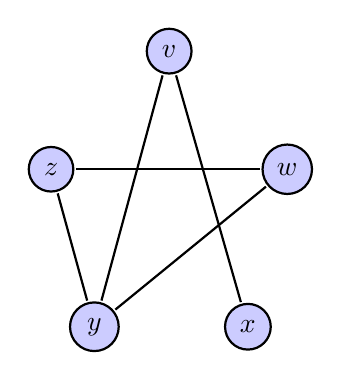
\begin{tikzpicture}[node distance=1cm,
                                 thick,main node/.style={circle,fill=blue!20,draw,outer sep=1pt}
                                ]           
               \node[main node] (1) at (0,0) {$z$};
               \node[main node] (2) at (1.5,1.5) {$v$};
               \node[main node] (3) at (3,0) {$w$};
               \node[main node] (4) at (2.5,-2.00) {$x$};
               \node[main node] (5) at (0.55,-2.00) {$y$};       
            
               \path%
                 (1) edge node [right] {} (3)  %{} is where the edge value would go
                 (3) edge [right] node {} (5)
                 (5) edge [right] node {} (2)
                 (2) edge [left] node {} (4)
                 (5) edge [right] node {} (1);
           \end{tikzpicture}\\[5pt]

{\color{blue}

 Here are the  adjacency matrix $A_G$, and the  incidence matrix $M_G$ of $G$
 using the vertices in the order $v,w,x,y,z$  and edges in the order $\{v,x\}, \{v,y\}, \{w,y\}, \{w,z\},\{y,z\}$:
 
 \[
  A_G=\left[
   \begin{matrix}
    0&0&1&1&0 \\ 
    0&0&0&1&1 \\ 
    1&0&0&0&0 \\ 
    1&1&0&0&1 \\ 
    0&1&0&1&0
   \end{matrix}
  \right]
  \qquad
  M_G=\left[
  \begin{matrix}
    1&1&0&0&0\\
    0&0&1&1&0 \\ 
    1&0&0&0&0 \\ 
    0&1&1&0&1 \\
    0&0&0&1&1
   \end{matrix}
  \right]
 \]
}           
\vfill\break

\item  For the graph below
 \begin{enumerate}
  \item  Find an eulerian circuit, or prove that none exists.\\[3pt]
  
 {\color{blue}
 We hope to construct a circuit in the graph that uses every edge of the graph exactly once. Note that repeated vertices are ok. One such a circuit is
 \[ 
 a\, b\, d\, e\, b\, c\, f\, e\, h\, f\, i\, h\, g\, d\, a\\[3pt]
 \] 
 }
  
  \item  Find a hamiltonian circuit or prove that none exists.\\[3pt]
{\color{blue}
We hope to construct a circuit (so the initial vertex  is the same as the terminal vertex) in the graph, with no repeated edges (but it's ok to omit some edges) which visits every vertex exactly once (except for  the initial vertex is the same as the terminal vertex).\\[2pt]
If there is a hamiltonian circuit, it will use exactly two edges at each vertex, and so the circuit must use both edges at vertices $a, c, i$ and $g$. That means we must use edges $\{a,b\}, \{b,c\}, \{c,f\}, \{f,i\},
\{i,h\}, \{h.g\}, \{g,d\},$ and $\{d,a\}$. Since we cannot use a third
edge from $b,f,h$ or $d$, there is no way to reach the vertex $e$.

Conclusion: There is no hamiltonian circuit.\\[5pt]
}
  
\end{enumerate}
 
 
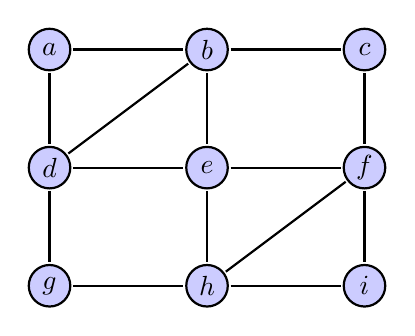
\begin{tikzpicture}[thick,
                       main node/.style={circle,fill=blue!20,draw,outer sep=1pt,
                                         inner sep=1pt,minimum size=15pt}
                      ] 
   \node[main node] (a) at (0.0,3.0) {$a$};
   \node[main node] (b) at (2.0,3.0) {$b$};
   \node[main node] (c) at (4.0,3.0) {$c$};
   \node[main node] (d) at (0.0,1.5) {$d$};
   \node[main node] (e) at (2.0,1.5) {$e$};
   \node[main node] (f) at (4.0,1.5) {$f$};
   \node[main node] (g) at (0.0,0.0) {$g$};
   \node[main node] (h) at (2.0,0.0) {$h$};
   \node[main node] (i) at (4.0,0.0) {$i$};
   \path%
    (a) edge [left] node {} (b)
    (a) edge [left] node {} (d)
    (b) edge [left] node {} (c)
    (b) edge [left] node {} (e)
    (b) edge [left] node {} (d)
    (c) edge [left] node {} (f)
    (d) edge [left] node {} (e)
    (d) edge [left] node {} (g)
    (e) edge [left] node {} (f)
    (e) edge [left] node {} (h)
    (f) edge [left] node {} (h)
    (f) edge [left] node {} (i)
    (g) edge [left] node {} (h)
    (h) edge [left] node {} (i);
  \end{tikzpicture}\\[5pt]
  
 \item  For the graph below
 \begin{enumerate}
  \item  Determine all the bridges.\\[3pt]
  {\color{blue} the bridges are $\{a,b\}$, $\{e,f\}$, and $\{g,h\}$.}\\[3pt]
  \item  Determine all the cut vertices.\\[3pt]
  {\color{blue} The cut vertices are $b,e,g,h$.}\\[5pt]
  
 \end{enumerate}
 
 
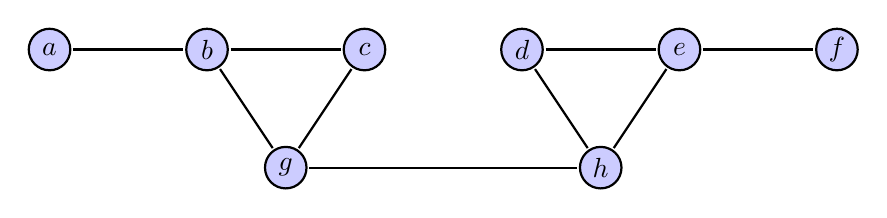
\begin{tikzpicture}[thick,
                       main node/.style={circle,fill=blue!20,draw,outer sep=1pt,
                                         inner sep=1pt,minimum size=15pt}
                      ] 
   \node[main node] (a) at (0.0,3.0) {$a$};
   \node[main node] (b) at (2.0,3.0) {$b$};
   \node[main node] (c) at (4.0,3.0) {$c$};
   \node[main node] (d) at (6.0,3.0) {$d$};
   \node[main node] (e) at (8.0,3.0) {$e$};
   \node[main node] (f) at (10.0,3.0) {$f$};
   \node[main node] (g) at (3.0,1.5) {$g$};
   \node[main node] (h) at (7.0,1.5) {$h$};
   
   \path%
    (a) edge [left] node {} (b)
    (b) edge [left] node {} (c)
    (d) edge [left] node {} (e)
    (e) edge [left] node {} (f)
    (b) edge [left] node {} (g)
    (c) edge [left] node {} (g)
    (d) edge [left] node {} (h)
    (g) edge [left] node {} (h)
    (e) edge [left] node {} (h);
  \end{tikzpicture}\\[5pt]


\item For each candidate degree sequence below, either draw a graph with that degree sequence or explain why that list cannot be the degree sequence of a graph.\\[3pt]

\begin{enumerate}

\item $4,4,4,4,4  $   \\[3pt]
{\color{blue}
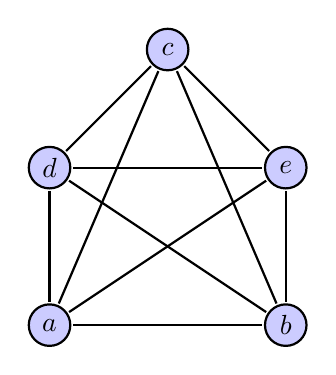
\begin{tikzpicture}[thick,
                       main node/.style={circle,fill=blue!20,draw,outer sep=1pt,
                                         inner sep=1pt,minimum size=15pt}
                           ] 
   \node[main node] (a) at (0.0,0.0) {$a$};
   \node[main node] (b) at (3.0,0.0) {$b$};
   \node[main node] (c) at (1.5,3.5) {$c$};
   \node[main node] (d) at (0.0,2.0) {$d$};
   \node[main node] (e) at (3.0,2.0) {$e$};
      \path%
    (a) edge [left] node {} (b)
    (a) edge [left] node {} (c)
    (a) edge [left] node {} (d)
    (a) edge [left] node {} (e)
    (b) edge [left] node {} (c)
    (b) edge [left] node {} (d)
    (b) edge [left] node {} (e)
    (c) edge [left] node {} (d)
    (c) edge [left] node {} (e)
    (d) edge [left] node {} (e);
      \end{tikzpicture}\\[5pt]
}

\item $6,4,4,4,4$\\[3pt]
{\color{blue} This graph is not possible since there are five vertices and so the maximum degree of a vertex is $4$. Remember that loops and multiple edges between vertices are not allowed.\\[5pt]
}

\item $0,0,0,0,0  $   \\[3pt]
{\color{blue}
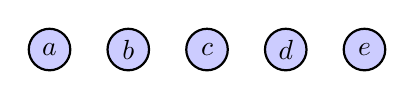
\begin{tikzpicture}[thick,
                       main node/.style={circle,fill=blue!20,draw,outer sep=1pt,
                                         inner sep=1pt,minimum size=15pt}
                      ] 
   \node[main node] (a) at (0.0,0.0) {$a$};
   \node[main node] (b) at (1.0,0.0) {$b$};
   \node[main node] (c) at (2.0,0.0) {$c$};
   \node[main node] (d) at (3.0,0.0) {$d$};
   \node[main node] (e) at (4.0,0.0) {$e$};
 \end{tikzpicture}\\[5pt] 
}

\item $3,2,1,1,1  $   \\[3pt]
{\color{blue}
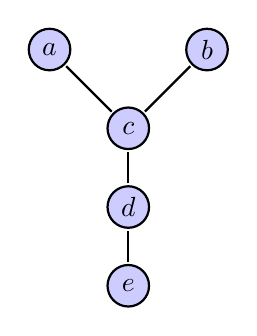
\begin{tikzpicture}[thick,
                       main node/.style={circle,fill=blue!20,draw,outer sep=1pt,
                                         inner sep=1pt,minimum size=15pt}
                           ] 
   \node[main node] (a) at (-1.0,3.0) {$a$};
   \node[main node] (b) at (1.0,3.0) {$b$};
   \node[main node] (c) at (0.0,2.0) {$c$};
   \node[main node] (d) at (0.0,1.0) {$d$};
   \node[main node] (e) at (0.0,0.0) {$e$};
      \path%
    (c) edge [left] node {} (a)
    (c) edge [left] node {} (b)
    (d) edge [left] node {} (c)
    (e) edge [left] node {} (d);
      \end{tikzpicture}\\[5pt]
}


\item $3,3,2,2,1  $   \\[3pt]
{\color{blue}
This graph is not possible since $3+3+2+2+1 = 11$ and the sum of the degrees of the vertices in a graph has to be even.\\[5pt]
}

\end{enumerate}



\item A {\it forest} is a graph consisting of one or more (separate) trees. If the total number of vertices in a forest is $f$, and the number of trees in the forest is $t$, what is the total number of edges in the forest?\\[3pt]

{\color{blue}
Suppose there are $t$ trees in the forrest. Let  $v_{1}, v_{2},\ldots, v_{t}$ be the number of vertices of tree $1$ through tree $t$, and let $e_{1}, e_{2},\ldots,e_{t}$ be the numbers of edges in tree $1$ through tree $t$. We know that, for each $i = 1,2, \ldots,t$, $e_{i} = v_{i} -1$. Adding those values from $i=1$ to $t$ gives
\begin{align*}
e_{1} + e_{2}+ \cdots +e_{t} &= (v_{1} -1)+(v_{2}-1)+\cdots+(v_{t}-1)\\
\text{total number of edges } &= (v_{1} + v_{2} + \cdots + v_{t}) - (1 + 1 + \cdots + 1)\\
\text{total number of edges } &= f -t.\\[5pt]
\end{align*}
}


\item (bonus) A tree is called {\bf star{-}like} if there is exactly one vertex with degree greater than $2$. How many different (that it, nonisomorphic) star{-}like trees are there with six vertices? (Note: If you draw the graph with the vertex of of degree greater than $2$ having the {\it arms} of the tree radiating out from it like spokes on a wheel, the name star{-}like will make sense.\\[3pt]

{\color{blue}
There are four different star{-}like trees with six vertices.

\vspace*{2\baselineskip}
\begin{minipage}[b]{0.1\textwidth}
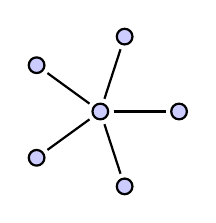
\begin{tikzpicture}[node distance=0.5cm,
                       thick,main node/.style={circle,fill=blue!20,draw,outer sep=2pt,inner sep=2pt}
                      ] 
  \node[main node] (f) at (0.00,0.00) {};
  \node[main node] (a) at (1.0,0.0) {};
  \node[main node] (b) at ( {cos(72)}, {sin(72)} ) {};
   \node[main node] (c) at ({cos(2*72)},{sin(2*72)}) {};
  \node[main node] (d) at ({cos(3*72)},{sin(3*72)}) {};
  \node[main node] (e) at ({cos(4*72)},{sin(4*72)}) {};
 
  \path%
   (f) edge [left] node {} (a)
   (f) edge [left] node {} (b)
   (f) edge [left] node {} (c)
   (f) edge [left] node {} (d)
   (f) edge [left] node {} (e);                   
  
 \end{tikzpicture}
 \end{minipage}
\hspace*{0.1\textwidth}
\begin{minipage}[b]{0.1\textwidth}
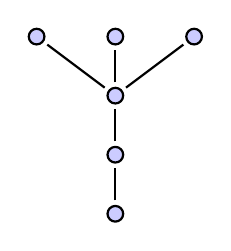
\begin{tikzpicture}[node distance=0.5cm,
                       thick,main node/.style={circle,fill=blue!20,draw,outer sep=2pt,inner sep=2pt}
                      ] 
  \node[main node] (g) at (0.00,0.00) {};
  \node[main node] (h) at (0.00,0.75) {};
  \node[main node] (i) at (0.00,1.50) {};
  \node[main node] (j) at (0.00,2.25) {};
  \node[main node] (k) at (-1.00,2.25) {};
  \node[main node] (l) at (1.00,2.25) {};
    \path%
      (g) edge [left] node {} (h)
      (h) edge [left] node {} (i)
      (i) edge [left] node {} (j)
      (i) edge [left] node {} (k)
      (i) edge [left] node {} (l);
   \end{tikzpicture}
   \end{minipage}
\hspace*{0.1\textwidth}
\begin{minipage}[b]{0.1\textwidth}
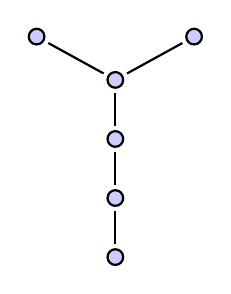
\begin{tikzpicture}[node distance=0.5cm,
                       thick,main node/.style={circle,fill=blue!20,draw,outer sep=2pt,inner sep=2pt}
                      ] 
  \node[main node] (g) at (0.00,0.00) {};
  \node[main node] (h) at (0.00,0.75) {};
  \node[main node] (i) at (0.00,1.50) {};
  \node[main node] (j) at (0.00,2.25) {};
  \node[main node] (k) at (-1.00,2.80) {};
  \node[main node] (l) at (1.00,2.80) {};
  

  \path%
      (g) edge [left] node {} (h)
      (h) edge [left] node {} (i)
      (i) edge [left] node {} (j)
      (j) edge [left] node {} (k)
      (j) edge [left] node {} (l);
   \end{tikzpicture}
   \end{minipage}
   \hspace*{0.1\textwidth}
\begin{minipage}[b]{0.1\textwidth}
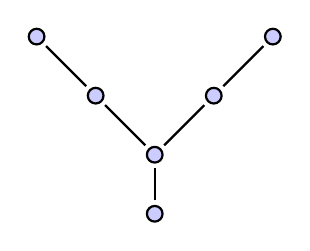
\begin{tikzpicture}[node distance=0.5cm,
                       thick,main node/.style={circle,fill=blue!20,draw,outer sep=2pt,inner sep=2pt}
                      ] 
  \node[main node] (m) at (0.00,0.00) {};
  \node[main node] (n) at (0.00,0.75) {};
  \node[main node] (o) at (-0.75,1.5) {};
  \node[main node] (p) at (0.75,1.5) {};
  \node[main node] (q) at (-1.50,2.25) {};
  \node[main node] (r) at (1.50,2.25) {};
  

  \path%
      (m) edge [left] node {} (n)
      (n) edge [left] node {} (o)
      (o) edge [left] node {} (q)
      (n) edge [left] node {} (p)
      (p) edge [left] node {} (r);
   \end{tikzpicture}
   \end{minipage}
}      

\end{enumerate}

\vfill\break
\section{Lesson 21: Test \#3}

\begin{center}
Part I:  ($2\frac{1}{2}$ points each) \underbar{True or False} (circle your answer): 
\end{center}
\vskip 10pt


\begin{enumerate}



\item  {\bf {\color{red}True} \ \  False}: $322\equiv -44 (\bmod\,  3 )$.
\vfill

\item  {\bf {\color{red}True} \ \  False}:  The congruence equation $12x \equiv 4 (\bmod\,88)$ has exactly
\vskip -1pt\hskip 80pt four solutions modulo $88$.
\vfill
 
\item  {\bf {\color{red}True }\ \  False}:  $\displaystyle\binom{25}{10} = \binom{25}{15} $.
 
\vfill
  
\item  {\bf True \ \  {\color{red}False}}:  When $(2x-1)^{30}$ is expanded, the coefficient of $x^{10}$ is 
$\displaystyle\binom{30}{10}$.

\vfill

\item  {\bf True \ \ {\color{red}False}}:   If $A$ and $B$ are finite sets, then $|A\cap B|$ is always less than or equal to $|A|-|B|.$ 
 \vfill
 
\item  {\bf {\color{red}True} \ \  False}:  $7018$ days after a Monday is a Friday.
\vfill
 
\item  {\bf True \ \ {\color{red} False}}: In a group of $200$ people, we can be sure there are at least 
\vskip -1pt\hskip 80pt $30$ born on the same day of the week.

\vfill
 
\item  {\bf True \ \ {\color{red} False}}: The characteristic roots for the recurrence $a_{n} = 3a_{n-1}+2a_{n-2}$
are $r = 1,2$. 
\vfill
  
\item  {\bf {\color{red}True} \ \  False}:  $a_n = n^2$ is a solution to the recurrence $a_0 = 0$ and for $n\geq 1$,
\vskip -1pt\hskip 80pt  $a_n = a_{n-1} + 2n-1$.
 
 \vfill
 
\item  {\bf {\color{red}True} \ \  False}: There is a graph with degree sequence $1,2,2,3$.

\vfill

\item  {\bf {\color{red}True} \ \  False}: The number of strings of five letters from the usual alphabet if repeats are
\vskip -1pt\hskip 83pt  not allowed is $\displaystyle {{26!}\over{21!}}$.

\vfill

\item  {\bf True \ \ {\color{red} False}}:  The number of ways of picking a subset of $\{a,b,c\cdots,z,0,1,2\cdots 9\}$
 consisting
\vskip -1pt\hskip 80pt   two elements is $\displaystyle {{26}\choose{2}} + {{10}\choose{2}}$.

\end{enumerate}

 \vfill
 \break
 
 
 
 
\begin{center} 
Part II: (5 points each) \underbar{Multiple Choice} (circle your answer):
\end{center}

\vfill

1) Recall that $K_n$ is the graph with $n$ vertices with every pair of vertices adjacent \vskip -1pt\hskip 12pt  (the complete graph on $n$ vertices). Circle all $n$ for which $K_{n}$ has a eulerian circuit.
\vskip 5pt
    \hskip 20pt {\color{red}(a) 3 }\hfill
\vskip 5pt
\hskip 20pt (b) 4\hfill
\vskip 5pt
    \hskip 20pt {\color{red} (c) 5}\hfill
\vskip 5pt
\hskip 20pt (d) 6\hfill
\vskip 5pt
\hskip 20pt {\color{red} (e) 7}\hfill

\vfill


2) When $35^{25}$ is divided by $17$, the remainder is

\vskip 5pt
\hskip 20pt (a) $0$\hfill
\vskip 5pt
\hskip 20pt {\color{red}(b) $1$}\hfill
\vskip 5pt
\hskip 20pt (c) $2$\hfill
\vskip 5pt
\hskip 20pt (d) $3$\hfill
\vskip 5pt
\hskip 20pt (e) None of the above.\hfill

\vfill

3) The number of different poker hands ($5$ cards, order not important, selected from a $52$ card
\vskip -1pt\hskip 12pt deck) with $3$ red cards and $2$ black cards is:

\vskip 5pt
\hskip 20pt {\color{red}(a) $\displaystyle{{26}\choose{3}}{{26}\choose{2}}$}\hfill
\vskip 5pt
\hskip 20pt (b) $\displaystyle{{52}\choose{5}} - {{26}\choose{23}}{{26}\choose{24}}$\hfill
\vskip 5pt
\hskip 20pt (c) $\displaystyle{{26}\choose{3}}+{{26}\choose{2}}$
\vskip 5pt
\hskip 20pt (d) $\displaystyle{{52}\choose{5}} - {{26}\choose{23}}-{{26}\choose{24}}$\hfill
\vskip 5pt
\hskip 20pt (e) None of the above.\hfill

 
\vfill


4) The number of strings of length $10$ of the $26$ letters that either begin with $a$ or end with $z$
\vskip -1pt\hskip 12pt is  

\vskip 5pt
\hskip 20pt (a) $2(26^8)$\hfill
\vskip 5pt
\hskip 20pt (b)  $26^8$\hfill
\vskip 5pt
\hskip 20pt (c) $26^9 + 26^9$\hfill
\vskip 5pt
\hskip 20pt (d) $(26^9)(26^9)$\hfill
\vskip 5pt
\hskip 20pt {\color{red}(e) None of the above.}\hfill

\vfill
\break

5)  In a listing of the five equivalence classes modulo $5$, four of the values
are $-11$, $8$, $100$, and
\vskip -1pt\hskip 12pt $32$. The last value could be

\vskip 5pt
\hskip 20pt (a) $0$\hfill
\vskip 5pt
\hskip 20pt {\color{red}(b) $1$ }\hfill
\vskip 5pt
\hskip 20pt (c) $2$\hfill
\vskip 5pt
\hskip 20pt (d) $3$\hfill
\vskip 5pt
\hskip 20pt (e) $4$\hfill

\vfill

6) The number of strings of length $10$ from the alphabet $\Sigma=\{a,b,c,d\}$ that contain
at least
\vskip -1pt\hskip 12pt  one $d$ is

\vskip 4pt
\hskip 20pt (a) $10^4-9^3$\hfill
\vskip 4pt
\hskip 20pt (b) $10^4 - 9^4$\hfill
\vskip 4pt
\hskip 20pt (c) $10^4-10^3$\hfill
\vskip 4pt
\hskip 20pt (d) $4^{10} - 3^9$\hfill
\vskip 4pt
\hskip 20pt {\color{red}(e) $4^{10}-3^{10}$}\hfill

\vfill

7)  I. M. N.  Oddman climbs stairs by taking either one  or three steps at a time.  
A recursive 
\vskip -1pt\hskip 12pt (along with initial terms $a_{0}=1$, $a_{1}= 1$, and $a_{2}= 1$)
formula for the number of
\vskip -1pt\hskip 12pt  different ways he can climb a
flight of $n$ steps is:
\vskip 3pt
\hskip 20pt (a) $a_n = a_{n-1} + a_{n-2}$\hfill
\vskip 3pt
\hskip 20pt {\color{red}(b) $a_n = a_{n-1} +a_{n-3}$}\hfill

\vskip 3pt
\hskip 20pt (c) $a_n = a_{n-2}+a_{n-3}$\hfill
\vskip 3pt
\hskip 20pt (d) $a_n = (a_{n-1} -1) + (a_{n-2} -2)$\hfill
\vskip 3pt
\hskip 20pt (e) $a_n = (a_{n-1}-1) + (a_{n-3}-3)$\hfill

\vfill

8) When looking for a particular solution to the recurrence $a_n = 2a_{n-1} + a_{n-2} + 2^n + 1$
your 
\vskip -1pt\hskip 12pt first try should be

\vskip 3pt
\hskip 20pt (a) $a_n = 2^n + B$\hfill
\vskip 3pt
\hskip 20pt (b) $a_n = A(2^n) + 1$\hfill
\vskip 3pt
\hskip 20pt {\color{red}(c) $a_n = A(2^n) + B$}\hfill
\vskip 3pt
\hskip 20pt (d) $a_n = A(2^n) + B(-2)^n + 1$\hfill
\vskip 3pt
\hskip 20pt (e) $a_n = A(2^n) + B(-2)^n + C$\hfill

\vfill
\break
\begin{center}
Part III. ($10$ points each) \underbar{Problems} 
\end{center}

\underbar{\small Do any three of the following four problems. If you do all four, I'll count your best three.}

\medskip

1)  Determine the number of permutations of all $10$ digits $\{0,1,2,3,4,5,6,7,8,9\}$ 
\vskip -1pt\hskip 12pt  (no repeats) if the digits $0$ and $1$ (in either order) must be adjacent. \\[3pt]

{\color{blue}
Arrange the $0$ and $1$: $2!$ ways to do that.\\
Arrange the nine items $2,3,4,5,6,7,8,9$ and the $01$ pair: $9!$ ways to do that.\\
Since we need to do both operations, the total number of {\itshape good} permutations is $2!\cdot 9!$.\\[5pt]
}




\vfill

2) You have inexhaustible supplies of red and blue marbles. The marbles are distributed\vskip-1pt\hskip15pt 
randomly,  one by one, into four tin cans. What is the minimum number of marble that \vskip-1pt\hskip15pt
have to be  distributed to be absolutely sure there is a can with three marbles of the\vskip -1pt\hskip 15pt
 same color.\\[3pt]
 
 {\color{blue}
 If there are five marbles in a tin can, some three must be the same color. \\
 So we need the least $n$
 so the $\lceil{\frac{n}{4}}\rceil = 5$. That is $n = 17$.\\[5pt]
 }

\vfill
\break

3) Determine a closed form formula for the sequence defined recursively by $a_0 = 0$, $a_1=1$,
\vskip -1pt\hskip 12pt and for $n\geq 2$, $a_n = a_{n-1} + 12a_{n-2}$.\\[3pt]

{\color{blue}
The characteristic equation is $r^2 -r-12 =0$. The left side factors as $(r+3)(r-4)$,
and so the characteristic roots are $r = -3,4$. The general solution is $a_n = A(-3)^n + B(4^n)$. Using the initial conditions, we get the system 
\begin{align*}
A+B = 0\\
-3A+4B = 1
\end{align*}
with solution $A = -\frac{1}{7}$ and $B = \frac{1}{7}$. So the closed form formula
is
\[
a_n = \frac{1}{7}(4^n) - \frac{1}{7}(-3)^m.
\]\\[5pt]
}



\vfill

4) Show the two graphs below are isomorphic by writing down a mapping (in other words, a pairing of the vertices) that is a graph isomorphism. Start with the pairing $a \to v$.\\[5pt]

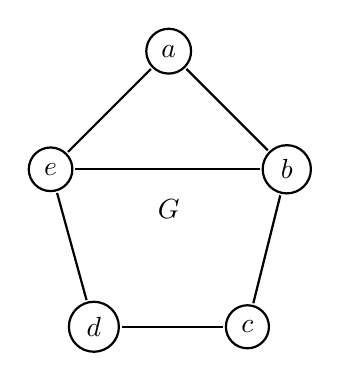
\begin{tikzpicture}[node distance=1cm,
                               thick,main node/.style={circle,draw,outer sep=1pt}
                              ]        
             \node[main node] (1) at (0,0) {$e$};
             \node[main node] (2) at (1.5,1.5) {$a$};
             \node[main node] (3) at (3,0) {$b$};
             \node[main node] (4) at (2.5,-2.00) {$c$};
             \node[main node] (5) at (0.55,-2.00) {$d$};
             \node (G) at (1.50,-0.50) {$G$};          
             \path%
               (1) edge node [right] {} (2)  %{} is where the edge value would go
               (2) edge [right] node {} (3)
               (3) edge [right] node {} (4)
               (4) edge [left] node {} (5)
               (5) edge [left] node {} (1)
               (1) edge [left] node {} (3);
         \end{tikzpicture}
         \hskip 1truein
         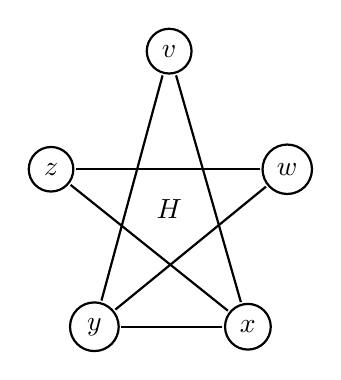
\begin{tikzpicture}[node distance=1cm,
                                 thick,main node/.style={circle,draw,outer sep=1pt}
                                ]           
               \node[main node] (1) at (0,0) {$z$};
               \node[main node] (2) at (1.5,1.5) {$v$};
               \node[main node] (3) at (3,0) {$w$};
               \node[main node] (4) at (2.5,-2.00) {$x$};
               \node[main node] (5) at (0.55,-2.00) {$y$};       
               \node (H) at (1.50,-0.50) {$H$};
               \path%
                 (1) edge node [right] {} (3)  %{} is where the edge value would go
                 (3) edge [right] node {} (5)
                 (5) edge [right] node {} (2)
                 (2) edge [left] node {} (4)
                 (4) edge [left] node {} (1)
                 (4) edge [left] node {} (5);
           \end{tikzpicture}\\[3pt]
           
           {\color{blue}
           
           There are two correct answers:
         
         \begin{align*}
           a\to v \qquad\qquad &a\to v\\
           b\to x \qquad\qquad &b\to y\\
           c\to z \qquad\qquad &c\to w\\
           d\to w \qquad\qquad &d\to z\\
           e\to y \qquad\qquad &e\to x\\
         \end{align*}
          }


\vfill



\end{document}

\bye